\cleardoublepage %poner esta linea al inicio de cada capitulo

\chapter{Introducción}

La agricultura ha sido uno de los pilares más importantes tanto para el desarrollo de la sociedad como para su manutención, ya que es gracias a está, que los países pueden generar empleos y aumentar sus recursos económicos, sin embargo las tareas de agricultura pueden llegar a ser tediosas o muy pesadas para las personas, es por esto que con el avance tecnológico se ha buscado mejorar el sector de la agricultura no solo para facilitar a los agricultores las tareas que deben hacer, sino también permitir que el producto ofrecido sea de mayor calidad, para garantizar que su comercialización tenga un mayor auge globalmente.\\

Uno de los principales avances tecnológicos en el sector agro-industrial, es la implementación de visión artificial en los procesos productivos, con esta se busca corregir las fallas humanas y garantizar que el producto mantenga siempre una buena y mejor calidad, que se busca garantizar con la normativa INCONTEC, la cual debe tener en cuenta para la exportación de productos agrícolas. El proyecto busca desarrollar un sistema mecatrónico implementando técnicas de visión artificial para mejorar el proceso de producción de la papa, esto podría ayudar al crecimiento del sector papicultor del país, debido a que se espera mejorar la calidad del producto y sea más eficiente su clasificación.


\newpage
\section{Objetivos}

\subsection{Objetivo General}

Implementar un prototipo para la clasificación de características de calidad en los tubérculos de papa producidos en la región Andina de Colombia, mediante técnicas de visión por computadora.

\subsection{Objetivos Específicos}
\begin{enumerate}
	\item Identificar a través de técnicas de visión artificial los rasgos de calidad "y características físicas" que se encuentran en los tubérculos de papa. 
	\item Evaluar el desempeño del prototipo propuesto para realizar la clasificación de los tubérculos de papa bajo las categorías de tamaño grande mediana y pequeña establecidas por la norma NTC341. 
	\item Comparar la precisión del modelo propuesto con modelos similares de clasificación
\end{enumerate}

\section{Alcances y Limitaciones}

\subsection{Alcances}

Para la realización del proyecto se debe tener en cuenta que se enfocará en los tubérculos de papa R12 y pastusa producidos en la región andina de Colombia. Se espera que el producto se encuentre limpio de suciedades como tierra y raíces, para llevar acabo el análisis por técnicas de visión artificial. El análisis se enfocará en identificar las características de calidad del producto para ser comercializado. Se propone un sistema mecatrónico tipo banda transportadora, para generar el desplazamiento de los tubérculos de papa por debajo de una cámara, que realiza el análisis de visión artificial y extrae las características de calidad de la papa.  

\subsection{Limitaciones}


El proyecto se encuentra limitado a los recursos de software y hardware, (computacionales), con los que cuentan los integrantes del proyecto y las plataformas open sources a las que se le puedan sacar provecho, para la implementación de los algoritmos que actualmente se encuentran en la literatura.

\section{Justificación}

En el proyecto se desarrollará un sistema mecatrónico, implementando técnicas de visión artificial para agilizar el proceso de producción de la papa, con el fin de mejorar el proceso actual que se lleva a cabo para la clasificación de calidad en los tubérculos de papa. El cultivo de la papa constituye el eje fundamental de la economía del país, en 283 municipios a nivel nacional, donde se involucran más de 90.000 familias principalmente en los departamentos de Boyacá, Cundinamarca, Antioquia y Nariño, los cuales concentran más del 85 \% de la producción \cite{referencia1}.
\\
\\
Actualmente, el reto que enfrenta el sector es el aumento de la calidad del producto, el rendimiento en producción y en consecuencia, incrementar el consumo. Debido a que la producción de papa en Colombia aporta el 3.3 \% del Producto Interno Bruto, (PIB), agropecuario, las siembras son de alrededor de 130 mil hectáreas y se cosechan cerca de 2,8 millones de toneladas, Además, en Colombia la producción de papa genera anualmente alrededor de 264.000 empleos, aproximadamente 75.000 son trabajos directos y alrededor de 189.000 son indirectos \cite{referencia2}.
Así, el presente trabajo permitirá mostrar los beneficios que trae la implementación de técnicas de visión artificial que podrían generar un  crecimiento al sector papicultor del país para competir con el mercado internacional.


\section{Descripción y formulación del problema}
La agricultura de Colombia es un componente fundamental en la economía del territorio, ya que juega un papel primordial en el desarrollo económico del país. Debido a que es la principal fuente de ingresos del área rural, hace un aporte relevante al desarrollo económico, la mitigación de la pobreza, y el desarrollo sustentable de Colombia.
\\
Uno de los sectores más grandes en la agricultura colombiana es el sector papicultor, en Colombia se caracteriza por tener poco desarrollo tecnológico y buscar abastecer el consumo interno, sin mayor exploración en mercados internacionales. Frente a la coyuntura en la que se encuentra el sector, gracias a los retos que traen consigo los acuerdos comerciales firmados por el gobierno nacional, el sector papicultor requiere urgentes transformaciones que permitan aumentar su competitividad y por ende lograr el crecimiento del sector.
\\
\\
Como consecuencia, en los últimos años, el sector agricultor de Colombia ha implementado herramientas tecnológicas que le permitan a los agricultores, aumentar la calidad de sus productos y así poder competir tanto en el mercado local como en el global. Pensando en esto, las diferentes técnicas de visión artificial, han tenido un auge en la agricultura de precisión, ayudando a clasificar productos basándose en sus diferentes características sin importar su clase, sin embargo, las técnicas de visión artificial no han sido aprovechadas para mejorar el sector papicultor colombiano.
\\
El sector agricultor de Colombia ha implementado diferentes técnicas de visión artificial, las cuales ayudan a clasificar los productos mediante las características que estos poseen, sin embargo, no se han implementado estas técnicas en la fase de almacenamiento de los tubérculos de papa, la cual es importante ya que en esta fase es donde se separan los tubérculos que cumplen las condiciones de calidad de los tubérculos que se encuentran defectuosos, ya que para la comercialización de este producto deben estar clasificados bajo la norma NTC 341.
\\ 
¿Cómo construir un prototipo para la clasificación de tubérculos de papa mediante técnicas de visión artificial?
\\
¿Qué tipo de proceso de clasificación permitirá agrupar los tubérculos de papa según sus características físicas y "patologías" mediante técnicas de visión artificial?	


\chapter{Marco Conceptual}
En este capitulo se van abordar algunos términos básicos necesarios, que ayuden al entendimiento y desarrollo del proyecto. 
\section{Agricultura de precisión} El término sobre el que se inspira la agricultura de precisión, es utilizar la porción adecuada de insumos, en el instante correcto y en el sitio preciso. La agricultura de precisión, (AP), implica la utilización de sistemas de posicionamiento universal, (GPS), y de otros medios electrónicos, para obtener datos del cultivo. Las tecnologías de la agricultura de precisión, permiten saciar una de las exigencias de la agricultura actualizada: el funcionamiento óptimo de enormes extensiones. Se muestra como primordial virtud, que la exploración de resultados de los ensayos se puede hacer por sectores diferentes en un mismo lote, y tal cual ajustar el desempeño diferencial en los mismos. La utilización de las tecnologías de la agricultura de precisión puede contribuir a mejorar los márgenes, por medio de un incremento del costo del rendimiento, (cantidad o calidad), de una reducción en la proporción de insumos, o de los dos paralelamente.
\\
\section{Artificial Neural Networks} Las RNA son sistemas de procesamiento de la información, cuya composición y manejo permanecen inspirados en las redes neuronales biológicas. Consisten en un enorme conjunto de recursos básicos de procesamiento, denominados nodos o neuronas, que permanecen organizados en capas. De esta forma, las RNA son sistemas adaptativos que aprenden de la vivencia, en otros términos, aprenden a realizar ciertas labores por medio de un entrenamiento con ejemplos ilustrativos.
\\ 
\section{DATA AUGMENTATION}

El Data augmentation consiste en la transformación de los datos existentes, para crear un \textit{dataset} con mayor cantidad de datos diferentes. El objetivo de esta herramienta es crear nuevos datos que puedan ser añadidos al conjunto ya existente, y así contar con más muestras para un mejor desempeño del algoritmo. Además de esto, también es implementado para reducir el \textit{overfitting}, ya que al añadir más información al conjunto de entrenamiento se evita que el modelo se sobre ajuste. \\


El concepto Data Augmentation tiene relación con los procedimientos para edificar algoritmos iterativos de mejora o muestreo, por medio de la introducción de datos no vigilados o cambiantes latentes. Para los algoritmos estocásticos, el procedimiento se popularizó en la literatura estadística por el algoritmo de incremento de datos de Tanner y Wong y en la literatura de física por el algoritmo de Swendsen y Wang, para el muestreo de los modelos de Ising y Potts y sus generalizaciones; en la literatura de física, el Data Augmentation, se conoce como el procedimiento de las cambiantes auxiliares. Generalmente, no obstante, la obra de esquemas de el Data augmentation es que den sitio a algoritmos básicos y rápidos, debido a que las tácticas famosas varían de una manera significativa con respecto a los modelos.\cite{van2001art}


\section{Imagen Binaria} Se define una imagen binaria como una función de dos variables discretas
a[m,n] las cuales puede tomar dos valores, ‘0’ o ‘1’, dependiendo del nivel de gris de la
imagen (una imagen binaria tiene dos niveles: blanco y negro). Existe una definición alternativa si consideramos que una imagen consiste en un conjunto de
coordenadas discretas (también pueden ser reales pero no es el objetivo de este estudio). En este sentido, el conjunto corresponde a todos aquellos puntos o píxeles que pertenecen a la imagen. Por lo tanto, se puede decir que en morfología matemática los conjuntos representan objetos en una imagen.
\\ 

\section{ISO 800} ISO no es más que la sensibilidad del sensor en el momento de captar la luz. Mayor número de ISO, más grande capacidad para captar luz y menor costo, menor capacidad para capturar esa luz. Una vez se duplica el costo ISO, o sea, se pasa de, ejemplificando, ISO 100 a ISO 200, se necesita la mitad de luz para poder hacer la misma exposición.
\\ 

\section{Procesamiento de imagenes} El procesamiento de imágenes, tiene como fin mejorar el aspecto de las imágenes y hacer más evidentes en ellas, ciertos detalles que se quieren hacer percibir. La imagen puede haber sido generada de muchas posibilidades, ejemplificando, fotográficamente, o electrónicamente, mediante monitores de televisión. El procesamiento de las imágenes se puede hacer mediante procedimientos ópticos, o bien mediante procedimientos digitales, en una PC. En la siguiente parte describiremos bastante brevemente dichos 2 procedimientos, sin embargo, previamente se va a hacer una síntesis simple de los principios matemáticos implícitos en los dos procedimientos, donde el teorema de Fourier es el eje central.
\\ 

\section{Reconstrucción morfológica} La re-composición morfológica, se puede tener en cuenta conceptualmente como dilataciones reiteradas de una imagen, denominadas, hasta que el contorno de la imagen del marcador se adapta bajo una segunda imagen, llamada imagen de máscara. En la re-composición morfológica, los picos de la imagen del marcador "se alargan"  o se dilatan.
\\ 

\section{Tubérculos de papa} La papa o patata es un tubérculo que se puede comer, se extrae de la planta herbácea americana Solanum Tuberosum, de procedencia andino. Es una planta correspondiente a el núcleo familiar de las solanáceas, procedente de Suramérica y cultivada por todo el planeta por sus tubérculos víveres. Ha sido domesticada en el altiplano andino por sus pobladores entre el 8500 y el 5000 a. n. e., y después ha sido llevada a Europa por los colonizadores españoles como una curiosidad botánica más que como una planta alimenticia. Su consumo ha ido creciendo y su cultivo se expandió a todo el planeta, hasta transformarse actualmente en uno de los más importantes alimentos para la gente.
\\ 

\section{Visión artificial} La perspectiva artificial ayuda a la industria a mejorar los procesos de producción por medio de imágenes digitales, con ellas se optimiza el control de calidad de aplicaciones industriales y de robots. Los sistemas de perspectiva examinan y se aseguran de conseguir los requisitos mínimos de calidad exigidos por cada fabricante. A lo largo del proceso de inspección, los sistemas de perspectiva informan de los probables errores detectados, lo cual posibilita un mejor control del proceso de producción.

\chapter{Estado del arte}

	El objetivo de los antecedentes, es analizar y realizar una revisión literaria sobre lo  que  se  ha hecho  a  nivel  teórico  y  práctico  en  cuanto a  la visión artificial en agricultura de precisión.  Además,  determinar  cuáles son los aportes que éstos le puedan dar a este trabajo de investigación.


\section{MatLab.}

	Comenzando por la literatura con temática en el procesamiento de imágenes, se tiene el trabajo de textit{J. porras, M. De La Cruz y A. Morian} \cite{article3}, en donde se menciona que la implementación de MATLAB\textsuperscript{\textregistered} como una herramienta de procesamiento de imágenes, radica en su facilidad para realizar cambios a las imágenes, es por esto qué diseñó un sistema para la clasificación de objetos con base en su forma y color, usando métodos de visión artificial en MATLAB\textsuperscript{\textregistered}, con el uso de la librería \textit{ufm.dll}, para capturar y procesar imágenes. El artículo de \textit{C. Nandi} \cite{inproceedings} presenta una investigación en dónde se consiguió calcular el tamaño de diferentes mangos, estimando el área cubierta en una imagen binaria, (imagen digital que tiene únicamente dos valores posibles para cada píxel), con base en el número de píxeles, luego de ser procesadas las imágenes, se clasificaron implementando un algoritmo basado en \textit{fuzzy logic}, teniendo en cuenta 5 variedades diferentes de mangos y como referencias el color de la cascara, tamaño, defectos superficiales, forma, firmeza, peso y olor.\\

\section{Artificial Neural Networks.}
	En cuanto a la clasificación, se deben usar técnicas de visión artificial y en primer lugar, se revisó literatura  acerca de ANN, (\textit{Artificial Neural Networks}), como el trabajo de \textit{L. Pencue-Fierro y J. León Téllez} \cite{article2}, en donde se aborda una investigación hecha en Perú, en donde se aplicó visión artificial usando ANN como método de clasificación de las principales características extraídas de las frutas, que son derivadas del análisis de las superficies, tanto en su contenido cromático como en la cantidad y distribución de defectos externos. De igual forma, en el trabajo publicado en la revista textit{Multimedia Tools and Applications} \cite{Shrivastava2017}, donde presentaron un sistema de visión artificial que usa un enfoque de categorización simplificado con un elevado índice de exactitud. El propósito del sistema es clasificar los granos de trigo de las especies \textit{triticum aestivum} y \textit{triticum durum} según sus propiedades visuales, usando una ANN del tipo MLP, (\textit{Multilayer Perceptron}); las imágenes se obtienen por medio de una cámara que captura las propiedades de tamaño, color y textura de cada grano con el objeto de que sirvan de acceso al procedimiento de categorización. Otro trabajo es el publicado por \textit{Ksh. Robert Singh y Saurabh Chaudhury} \cite{Singh2016}, en donde se propone el uso de redes neuronales BPNN, (\textit{Back Propagation Artificial Neural Networks}), como método de clasificación y la descomposición mediante ondículas, (Tipo especial de transformada matemática que representa una señal en términos de versiones trasladadas y dilatadas de una onda finita), para clasificar los granos de arroz. El modelo de clasificación implemento una red neuronal BPNN de cuatro capas la cual presento mejores resultados en comparación con otros métodos.\\
	
	Por último, usando el método de clasificación ANN, se tiene el trabajo hecho por \textit{Krzysztof Koszela y Lukasz Gierz} \cite{Przybyl2019}, donde se presenta una forma para garantizar la correcta clasificación de los productos y reducir las pérdidas durante su almacenamiento. La investigación abarca esfuerzos centrados en la evaluación sensorial de patatas con el análisis de imágenes por ordenador y la modelización neuronal ANN. El objetivo de este estudio fue desarrollar un método para asistir a la identificación de cualquiera de las variedades y la turgencia de los tubérculos de patata, (Fenómeno que ocurre cuando una célula se dilata debido a la presión ejercida por los fluidos y por el contenido celular sobre las paredes de la célula), llevado a cabo sobre la base de los datos gráficos codificados en forma de imágenes digitales, obtenidos mediante algoritmos que interpretan los descriptores de imagen.\\

\section{Super Vector Machine.}
	Otro método de clasificación revisado en la literatura es el de SVM \textit{Super Vector Machine}), como el usado en el trabajo de \textit{Tao Liu} y otros investigadores \cite{LIU201679}, en donde realizaron un proceso para analizar granos de arroz. El procedimiento usa 4 fuentes de luz para crear la sombra del grano en 4 direcciones; la diferencia en medio de las siluetas de los granos llenos y no llenos, se evalúa por medio del estudio de imágenes y un clasificador SVM. El análisis se hace mediante el uso de imágenes RGB, (Red-Green-Blue), de los granos con las siluetas, luego se segmentan desde la imagen binaria, para sustraer información como el sector del grano y de la sombra. En el documento publicado por \textit{Chia-Lin}  y otros investigadoores \cite{CHUNG2016404}, se menciona un método para clasificar plántulas, (Embrión ya desarrollado como consecuencia de la germinación de una semilla), sanas e infectadas. Consiste en el análisis de imágenes mediante un escáner y el proceso de clasificación utilizando SVM, en donde se hace uso de dos clasificadores, el primero distingue entre las plantas sanas y contaminadas, por otra parte, el segundo mide los niveles de contaminación. En el trabajo de \textit{Rillian Diello y Lucas Pires} \cite{PIRES201648}, se propuso un método de detección automática de enfermedad en cultivos de soja, el cual se basa en descripciones locales, conocido como el método BOV, (Bag of Values), luego de escanear la hoja. Se obtuvo a través de los vectores de entrada una clasificación en dos categorías, enfermo y sano, a partir de un clasificador SVM. Y por último, en este tipo de clasificador, el trabajo de \textit{Chengming Sun y Tao Liu} \cite{SUN2014426}, se propone un sistema para analizar el porcentaje de granos en el arroz que se encuentran en condiciones para ser distribuidos. El algoritmo se encarga de la división de los granos de manera automática. Tras la segmentación, es viable obtener el número de granos presentes en la imagen y la información específica, la exactitud del procedimiento puede verse afectada si el germen no se extrae del todo, por esa razón, el sistema detecta la viable región de germen y estima esta información usando SVM.\\

\section{Otros métodos}
	En la literatura se encontraron artículos que usaban más de un método de clasificación, un ejemplo es el trabajo hecho por \textit{Tao Liu y Wen Chen} \cite{LIU201682}, el cual puso en práctica un método para controlar la población de pulgones, (Familia de insectos hemípteros), en el trigo, usando los métodos SVM, el algoritmo MSER, (\textit{Maximally Stable Extremal Regions}), y el HOG, (\textit{Histogram of Gradients}). El uso de estos 3 métodos se conoce como SMH, (Unión entre SVM, MSER y HOG), se basa en el análisis de imágenes, tratadas a partir de unos parámetros, con la finalidad de detectar la presencia y/o ausencia de pulgones, se hizo uso de este método a partir del color y la densidad de población. Al comparar este método con otros cinco comúnmente utilizados, los resultados presentaron un rendimiento superior en la identificación de pulgones. \\
	
	De igual manera, el artículo de \textit{Rodica Sobolu} \cite{sobolu2020automatic}, propone un algoritmo de clasificación automática de patatas. Se realizaron dos tipos de clasificación: una en función del tamaño de las patatas y otra en función de su calidad. La segmentación de las zonas defectuosas se hizo mediante métodos como \textit{global thresholding}, para extraer características morfológicas y estadísticas de las zonas segmentadas. Estas características se eligieron como entradas para los algoritmos de clasificación, en donde se usaron los métodos SVM, \textit{Decision  Tree} y LDA, (\textit{Linear Discriminant Analysis}), implementados en MATLAB\textsuperscript{\textregistered} Classification Toolbox. Se llegó a la conclusión de que la SVM ha clasificado las patatas según su tamaño con una mayor tasa de éxito. En el caso de la clasificación por calidad, se recomienda el método LDA.\\
	
	Los anteriores son los métodos más comunes que se encontraron en la literatura investigada, sin embargo, hay unos métodos poco comunes como por ejemplo los presentados en el artículo de \textit{Alberto Martines Rodriguez} \cite{article5} en donde se identificaron objetos en movimiento mediante la ayuda de la visión artificial y la transmisión de datos a un brazo robótico implementando \textit{C++} y \textit{Open CV}, usando el código de cadena, (Actualmente el grupo de reconocimiento de patrones e inteligencia artificial aplicada), para calcular las características de los objetos por color y forma. También, el artículo hecho por \textit{L. Han y M. S. Haleem} \cite{7237209}, que se usa para la detección automática, fue necesario hacer uso inicialmente de separar el fondo de la hoja, para este proceso se usó el algoritmo MCW, (\textit{Marker-Controlled Watershed}). El SLIC, (\textit{Simple Linear Iterative Clustering}), se utilizó para obtener las características presentadas por la enfermedad sobre la planta y por ultimo, la clasificación y textura se obtienen a través de GLCM, (\textit{Gray Level Co-occurrence Matrix}), el modelo de clasificación fue el SVM, este método propuesto presento un mayor rendimiento.\\
	
	El último artículo revisado es presentado por \textit{Michael Barnes y Tom Duckett} el \cite{Barnes2010}, cuyo objetivo de  investigación es introducir un método automático de detección de manchas en imágenes digitales de patatas. El sistema desarrollado es entrenable, de modo que pueda trabajar con diferentes variedades de patatas y variaciones en las estaciones, condiciones de iluminación, etc. Otro objetivo, pensando en su posible implantación en entornos industriales, es permitir el procesamiento de imágenes en tiempo real, posiblemente mediante la construcción de \textit{Minimalist Boosted Classifier}, que extraigan un subconjunto mínimo de todas las características que optimicen el rendimiento de la detección con el menor coste computacional posible.





\chapter{Diseño Del Algoritmo de Clasificación}


Se diseñó un algoritmo de clasificación utilizando Redes Neuronales Convolucionales y técnicas de visión artificial con la librería \textit{Open CV}, para clasificar las características de tipo, daño y tamaño de tubérculos de papa. El Procedimiento que se llevó acabo se presenta en la Figura \ref{fig:flujogeneral}, cada ítem será explicado en las siguientes secciones. 


\begin{figure}[ht]
	\centering
	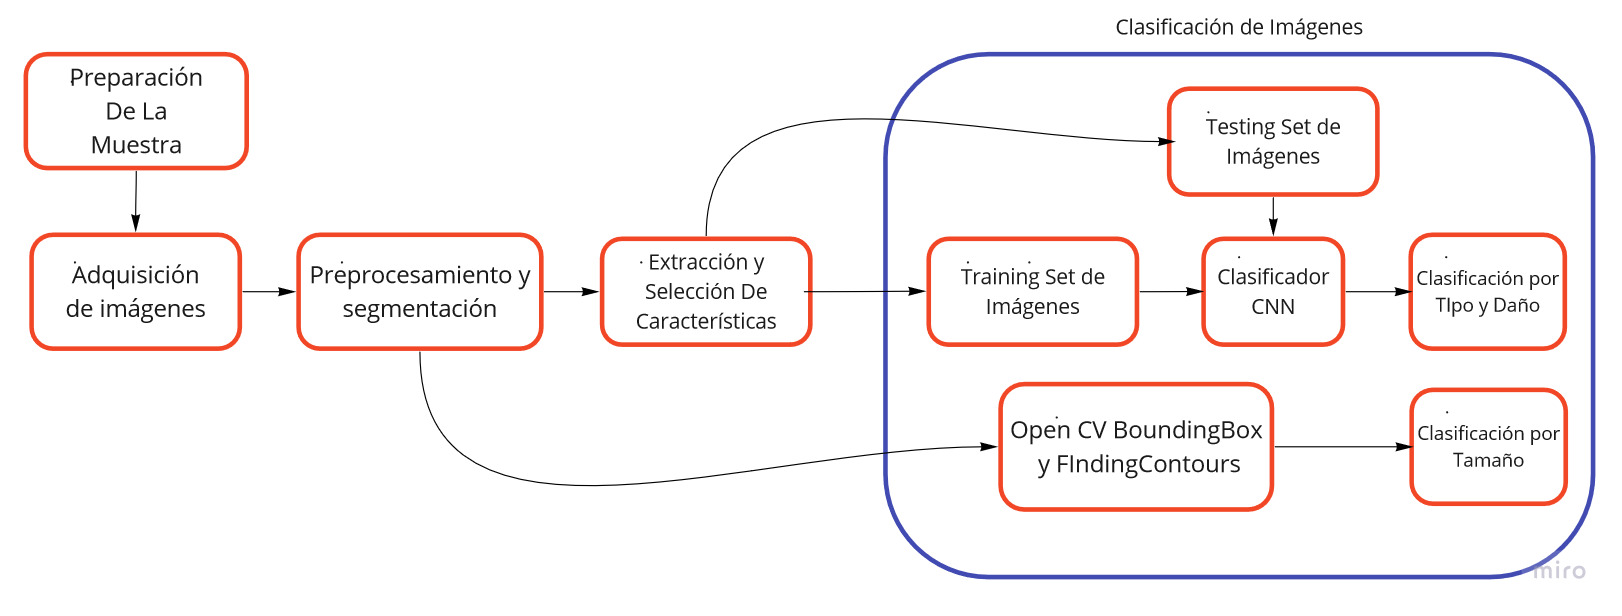
\includegraphics[scale=0.3]{Figs/FGGeneral.jpg}
	\caption{Arquitectura del Sistema de Clasificación}
	\label{fig:flujogeneral}
\end{figure}

El sistema propuesto para realizar la clasificación de tubérculos de papa en este documento, consiste desde la adquisición de muestras y creación de un dataset de tubérculos de papa, hasta el diseño de un algoritmo de clasificación con Redes Neuronales, utilizando la librería \textit{Pytorch} y la librería \textit{Open CV} de \textit{Python}. Será implementado en un prototipo de banda transportadora, que permita el movimiento de los tubérculos de papa para ser clasificados, mediante un microcontrolador y una cámara. Los sistemas de Visión Artificial que se destinan a realizar inspecciones visuales, permiten que el proceso sea más eficiente si requieren alta velocidad, gran aumento en cantidad de producción y en funcionamiento las 24 horas del día o la repetibilidad de las medidas \cite{artificial2012aplicacion}.


\section{Preparación y Adquisición De Las Imágenes}

	Se preparó un total de 592 tubérculos de papa, que manualmente fueron clasificados en tres categorías definidas. Las etiquetas de cada imagen se encuentran dentro del nombre de cada archivo, que corresponde al metadata de cada foto tomada. Definido de la siguiente manera:
	
	\begin{itemize}
		\item \textit{Tipo:} Pastusa o R12 $[0,1]$
		\item \textit{Daño:} Buena y Defectuosa $[0,1]$
		\item \textit{Tamaño:} Muy grande, Grande y Mediana $[0,1,2]$
		\item \textit{Numero de la Imágen} Etiqueta asignada por la cámara.
	\end{itemize}	
	
	Las fotos tomadas para la creación del \textit{Dataset}, poseen un tamaño de (3168, 4752) pixeles. Fueron tomadas con una cámara profesional \textit{Canon EOS 50D}, que tiene 15.1 mega pixeles de resolución y se puede ajustar la sensibilidad ISO desde 100 hasta 3200. La cámara fue configurada con ISO-800 que corresponde al parámetro de sensibilidad del sensor de ruido de la cámara, una velocidad de obturación de $\frac{1}{640}$ segundos, que corresponde al dispositivo que controla el tiempo en el que la luz incide sobre el sensor de la cámara, y finalmente una apertura de diafragma de $F 7.1$ que corresponde a la apertura del lente que deja pasar la luz \cite{Camara}, tener en cuenta que a mayor apertura de diafragma, menor luz se deja pasar. Se construyó una caja con iluminación fija la cual se muestra en la Figura \ref{fig:chamber} usando bombillos de luz blanca, de $6500$ Kelvin de temperatura de color, para que la iluminación en todas las fotos tomadas fuera uniforme, y la cámara fue fijada a un trípode ubicado a $30 \ cm$ de la base, para que la distancia del lente de la cámara con respecto a la muestra de papa fuera siempre la misma en las 592 fotos.

	\begin{figure}[ht]
		\centering
		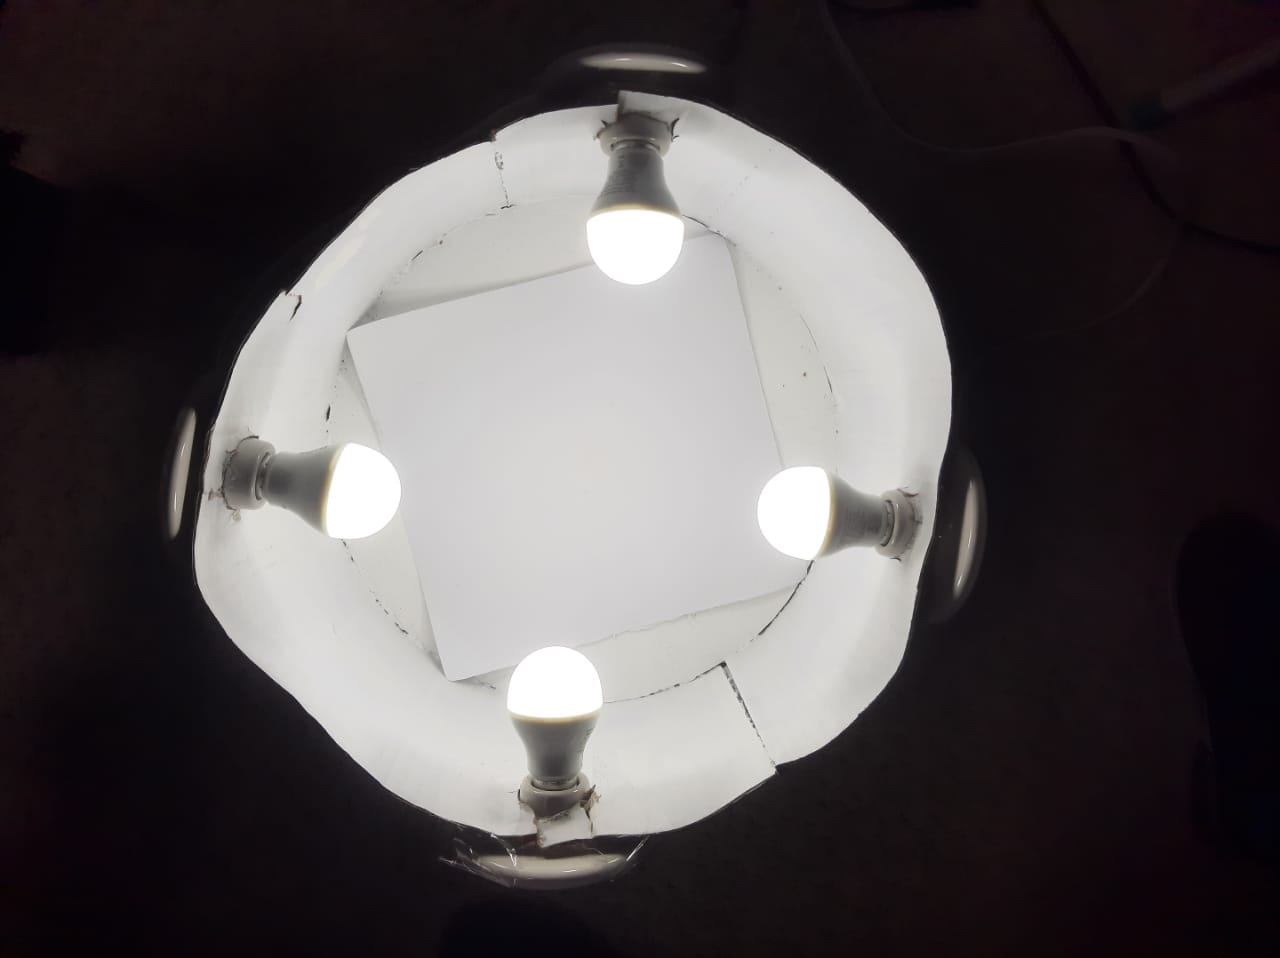
\includegraphics[scale=0.15]{Figs/Chamber.JPEG}
		\caption{Récamara Para la Toma de Fotos}
		\label{fig:chamber}
	\end{figure}
	
	Utilizando la librería \textit{Pandas} de \textit{Python}, se creó un \textit{Dataframe} que contiene el metadata de cada imagen. En la Tabla \ref{table:metadata} se puede apreciar la distribución del \textit{MetaData} de las imágenes almacenas en el \textit{Dataset}, donde se toman cinco imagenes al azar como muestra. A partir de esta tabla se crea un archivo \textit{.CSV} donde se encuentra la información de las 592 imágenes.
	
	\begin{table}[ht]
		\centering
		\begin{tabular}{|c|c|c|c|}
			\hline
			Tipo & Daño & Tamaño & Filename \\
			\hline
			R12 & Defectuosa & Grande & 1\_1\_1\_075.JPG \\
			\hline
			PASTUSA & Buena & Grande & 0\_0\_1\_1973.JPG \\
			\hline
			R12 & Buena & Grande & 1\_0\_1\_2054.JPG \\
			\hline
			PASTUSA & Buena & Mediana & 0\_0\_2\_2042.JPG \\
			\hline
			PASTUSA & Buena & Grande & 0\_0\_1\_1955.JPG \\
			\hline
		\end{tabular}	
		\caption{MetaData de 5 Imágenes de Muestra}
		\label{table:metadata}
	\end{table}


	Una vez la información de cada imagen fue guardada en el archivo \textit{metadata.csv}, se agruparon las posibles combinaciones de las características de \textit{Tipo} y \textit{Daño}, para definir las \textit{clases} dentro de la red neuronal. Para realizar este proceso, se creó una condición dentro del \textit{Dataframe}, que contiene el \textit{Metadata} para generar una columna adicional con la información de la Tabla \ref{table:Clases}.	
	
	\begin{table}[ht]
		\centering
		\begin{tabular}{|c|c|c|c|c|}
			\hline
			PASTUSA & R12 & Buena & Defectuosa & Clase \\
			\hline
			X &  & X &  & CLASE 1 \\
			\hline
			X &  &  & X & CLASE 2 \\
			\hline
			& X & X &  & CLASE 3 \\
			\hline
			& X &  & X & CLASE 4 \\
			\hline
		\end{tabular}	
		\caption{Clases Definidas}
		\label{table:Clases}
	\end{table}	

De esta forma se definieron las $4 \ clases$ que serán entrenadas en la red neuronal, para el posterior proceso de clasificación por visión artificial. 


\newpage
\section{Distribución del Dataset}
	  
	Para determinar la distribución total del dataset, con el uso de la librería \textit{Plotly}, se crearon gráficas para determinar el porcentaje de imágenes pertenecientes cada característica definida en el \textit{Dataset}. La Figura \ref{fig:distribuciontipo}
		
	\begin{figure}[ht]
		\centering
		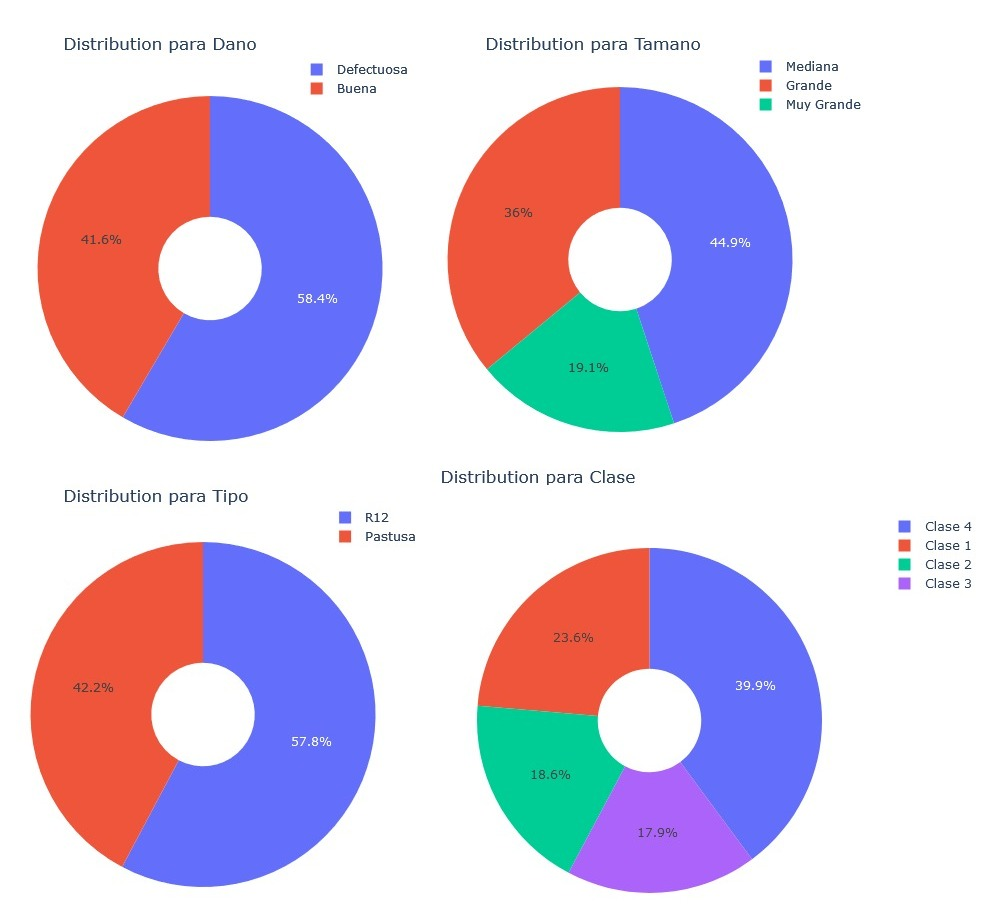
\includegraphics[scale=0.4]{Figs/Distribucion.jpg}
		\caption{Distribución del Dataset Según Sus Características Y Clases Definidas}
		\label{fig:distribuciontipo}
	\end{figure}

	Se definieron los \textit{Set's} de \textit{Train} y \textit{Test}, que fueron creados para el entrenamiento y validación de la red neuronal, a partir del archivo \textit{metadata.csv} de la Tabla \ref{table:metadata}. Se utilizó $80\%$ para \textit{Train} y $20\%$ para \textit{Test}. Se crearon los archivos \textit{train.csv} y \textit{test.csv} que contienen el \textit{metadata} y la dirección de las imágenes separadas en el respectivo $80\%$ y $20\%$.



\newpage
\chapter{Algoritmo de Clasificación}
En este capitulo se presenta la definicion y estructura de una red neuronal artificial convolucional, la preparación del dataset implementado durante el entrenamiento de la red neuronal y los diferentes modelos implementados en el desarrollo del proyecto.

	\section{Red Neuronal Artificial Convolucional}

	Se desarrolló una red neuronal artificial, (\textit{CNN}), para clasificar las características de tipo y daño, de los tubérculos de papas descritos en el \textit{Metadata} Tabla \ref{table:metadata}. La arquitectura general de una red artificial convolucional, (\textit{CNN}), se muestra en la Figura \ref{fig:cnnarchitecture} \cite{cnnarchitecture}. Se realizaron pruebas con las arquitecturas \textit{Alexnet}, \textit{Resnet18}, \textit{VGG11} y \textit{VGG19} y se implementó la optimización bayesiana en ciertos hiperparámetros de las arquitecturas existentes, para mejorar los resultados. 
	
	\begin{figure}[ht]
		\centering
		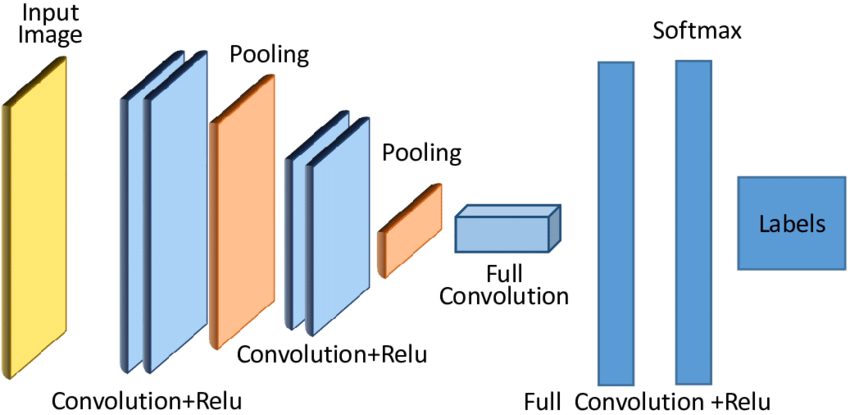
\includegraphics[scale=0.25]{Figs/A-generic-CNN-Architecture.png}
		\caption{Arquitectura General De Una CNN}
		\label{fig:cnnarchitecture}
	\end{figure}	
	
	El procedimiento realizado para desarrollar la red neuronal, se aprecia en la Figura \ref{fig:procedimiento}, donde se indica los pasos a seguir, previo a implementar alguna de las arquitecturas. Cada ítem será descrito en las próximas secciones.  


	\begin{figure}[ht]
		\centering
		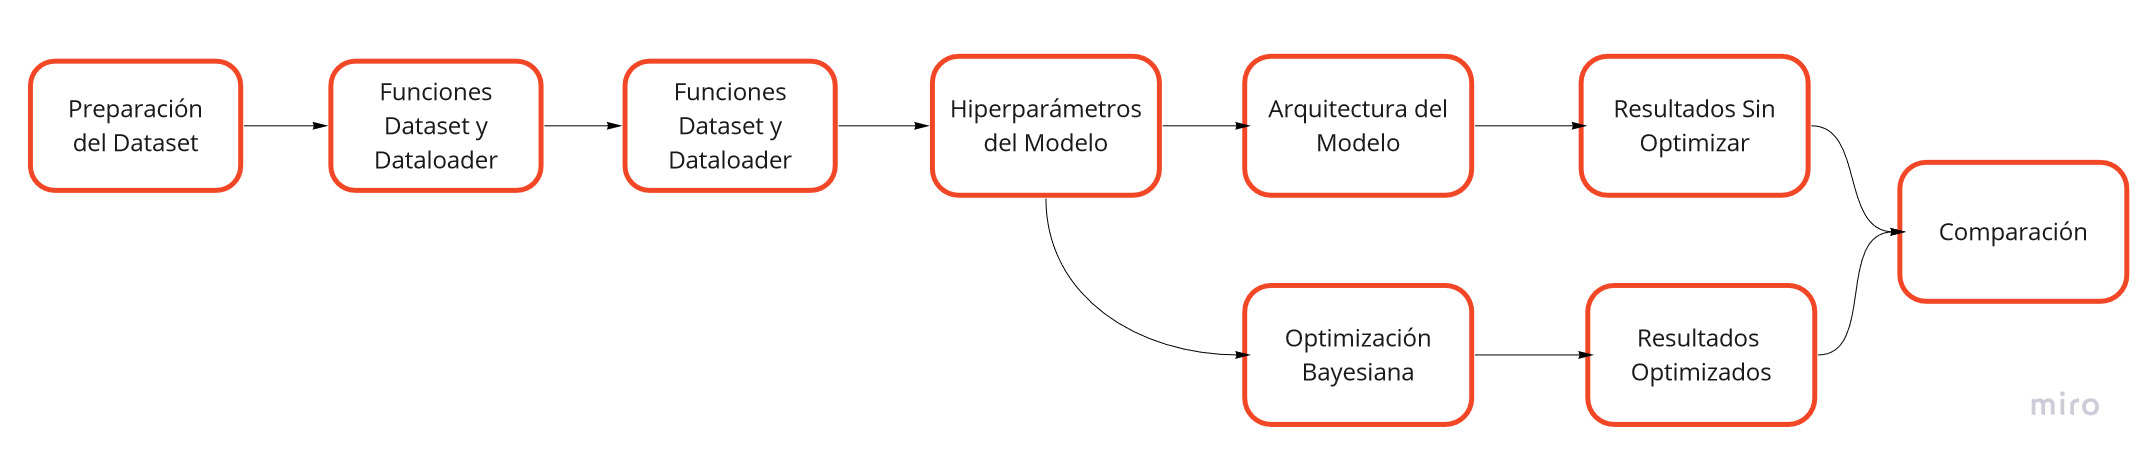
\includegraphics[scale=0.2]{Figs/procedimiento.jpg}
		\caption{Procedimiento Diseñado Para Implementar La \textit{CNN}}
		\label{fig:procedimiento}
	\end{figure}	


\newpage
		\subsection{Preparación Del \textit{Dataset}}
		En este apartado se explica como se lleva acabo el preprocesamiento de imágenes y los diferentes aplicados para la creación del Data Augmentation.
			\subsubsection{PREPROCESAMIENTO DE IMÁGENES}

			Usando el módulo \textit{torchvision.tranforms.compose()}, de la librería \textit{Pytorch}, se puede encadenar unas determinadas funciones que aplican diferentes tipos de filtros y transformaciones al \textit{Dataset}. De esta forma, se puede crear la tarea de segmentación debido a que las transformaciones aumentan en consideración el tamaño original del \textit{Dataset}, facilitando así, la extracción de características de cada imagen \cite{Pytorch}. Las transformaciones disponibles en éste módulo se presentan en la Tabla \ref{table:Filters1}.
			
			\begin{table}[ht]
				\centering
				\begin{tabular}{|p{4cm}|p{4cm}|p{4cm}|p{4cm}|}
					\hline
					Image Transform       & \multicolumn{1}{c|}{Use}                                                               & Image Transform       & \multicolumn{1}{c|}{Use}                                                                        \\ \hline
					CenterCrop            & Recorta la imagen en el centro                                                         & RandomResizedCrop     & Recorta una porción aleatoria de la imágen y la redimensiona a un tamaño determinado            \\ \hline
					ColorJitter           & Cambia aleatoriamente el brillo, el contraste, la saturación y el tono de una imagen   & RandomRotation        & Rota la imagen a un ángulo determinado                                                          \\ \hline
					FiverCrop              & Recorta la imagen en cuatro esquinas y el recorte central                              & RandomVerticalFlip    & Voltea verticalmente la imagen al azar con una probabilidad dada                                \\ \hline
					Grayscale             & Convierte la imágen en escala de grises                                                & Resize                & Redimensiona la imagen al tamaño dado                                                           \\ \hline
					Pad                   & Rellena la imágen en todos sus lados con el valor de "pad" dado                        & TenCrop               & Recorta la imagen dada en cuatro esquinas y el recorte central más la versión volteada de éstas \\ \hline
					RandomAffine          & Transformación afín aleatoria de la imagen manteniendo el centro invariante            & GaussianBlur          & Desenfoca la imágen con un filtro gausseano                                                                                                                                                     \\ \hline
				\end{tabular}
				\caption{Funciones de transformación de imágenes del módulo de \textit{Pytorch}}
				\label{table:Filters1}
			\end{table}
			
			En la Tabla \ref{table:Filters1} se observa una parte de las transformaciones de imágenes disponibles en el módulo \textit{torchvision.tranforms.compose} de la librería \textit{Pytorch}. En el caso del \textit{Dataset} de papas creado, se deben tener en cuenta únicamente las transformaciones cuyo resultado sea relevante para la extracción de características de la imágen, por ejemplo, como se explicó anteriormente, se va a clasificar el tubérculo de papá en tipo y daño, con la red neuronal, por este motivo, el color es una característica que define si la papa pertenece a la clase \textit{R12} o \textit{Pastusa} y, en algunos casos, si se encuentra con algún tipo de daño, por este motivo, los filtros que transforman la imágen en escala de grises no son relevantes y podrían afectar el rendimiento del algoritmo.
		
			\begin{table}[ht]
				\centering
				\begin{tabular}{|p{4.5cm}|p{3.5cm}|p{3.8cm}|p{3.5cm}|}
					\hline
					Image Transform       & \multicolumn{1}{c|}{Use}                                                               & Image Transform       & \multicolumn{1}{c|}{Use}                                                \\ \hline
					Randomcrop            & Recorta la imágen aleatoriamente                                                       & RandomInvert          & Invierte los colores de la imágen de forma aleatoria                    \\ \hline
					RaandomGrayscale      & Convierte la imágen en escala de grises aleatoriamente                                 & RandomPosterize       & Reduce el número de bits de cada canal de laa imágen de forma aleatoria \\ \hline
					RandomHorizontalFlip  & Voltea horizontalmente la imágen al azar con una probabilidad dada                     & RandomSolarize        & Invierte aleatoriamente el valor de los pixeles por encima de un umbral \\ \hline
					RandomPerspective     & Realiza una transformación de perspectiva aleatoria de la imagén                       & RandomAutocontrast    & Autocontraste de los píxeles de la imagen dada aleatoriamente           \\ \hline
					RandomAdjustSharpness & Ajusta la nitidez de la imágen de forma aleatoria                                      & RandomEqualize        & Equaliza el histograma de la imágen dada aleatoriamente                 \\ \hline
					RandomApply           & Aplicar aleatoriamente una lista de transformaciones con una probabilidad determinada. & \multicolumn{1}{l|}{} &                                                                         \\ \hline
				\end{tabular}
				\label{table:filters2}
				\caption{Funciones de transformación de imágenes del módulo de \textit{Pytorch}}
			\end{table}

			De igual forma, en la Tabla \ref{table:filters2}, se observan algunos filtros como recortes en la imágen, rotaciones, cambios de perspectiva, cambios en la nitidez y contraste de la imágen. Se escogieron los filtros considerados mejores, (NO cambian la morfología del color), para el caso del \textit{Dataset} de tubérculos de papa creado en este documento. 
			
			
			
			\newpage
			Los filtros que se utilizaron en el desarrollo del algoritmo de clasificación, teniendo en cuenta aquellas transformaciones que podrían afectar el rendimiento del algoritmo son:
			
			\begin{itemize}
				\item Resize
				\item ColorJitter
				\item RandomRotation
				\item GaussianBlur
				\item RandomPerspective
				\item RandomAdjustSharpness
			\end{itemize}

			Como se está utilizando la librería \textit{Pytorch}, las imágenes deben ingresar en formato \textit{Tensor}, que convierte los valores de los píxeles de una imágen \textit{PIL} estándar, con un rango de $[0, 255]$,  a un tensor decimal de \textit{Pythorch}, con valores en un rango con valores $[0.0, 1.0]$ de la forma  $(C, H, W)$, siendo C el número de canales de la imágen, (1 si es en escala de grises, 3 si es \textit{RGB}), $H$ y $W$ el tamaño de la imágen. \\
			
			Una vez la imágen está en formato \textit{PyTorch FloatTensor}, se decidió utilizar la función \textit{torchvision.tranforms.normalize()} para normalizar las imágenes. La normalización de una imágen consiste en modificar los valores del tensor, que se encuentran entre $[0.0, 1.0]$, para que el promedio y la desviación estándar sean $0$ y $1$ respectivamente. Para hacer esto se utiliza la Ecuación \ref{eq:normalize} \cite{Pytorch}
			
			\begin{equation}
				{output[Channel]=\frac{Input[Channel]-Mean[Channel]}{std[Channel]}}
				\label{eq:normalize}
			\end{equation}

			La normalización se utiliza debido a que ayuda a los datos a estar definidos dentro de un rango y reducir la asimetría entre ellos, lo que permite un aprendizaje más rápido. Se diseñó una función en \textit{Python} que calcula el promedio y la desviación estándar, para \textit{Trainset} y para el \textit{Testset}. De esta forma se garantiza que la normalización sea correcta en el total del \textit{Dataset}. Los valores obtenidos para el \textit{Trainset} Ecuación \ref{eq:meanstd1} y el \textit{Testset} Ecuación \ref{eq:meanstd2} respectivamente.
			
			\begin{equation}				{mean = [0.7467, 0.7389, 0.7432] \hspace*{1cm}  std  = [0.1288, 0.1633, 0.2045]}
				\label{eq:meanstd1}
			\end{equation}


			\begin{equation}
				{mean = [0.7507, 0.7430, 0.7486] \hspace*{1cm}  std  = [0.1265, 0.1609, 0.2012]}
				\label{eq:meanstd2}
			\end{equation}


			La Figura \ref{fig:agumentation} enseña una matriz de imágenes como parte del \textit{Trainset}, que muestra las transformaciones hechas al $80\%$ de las imágenes del \textit{Dataset}, y la clase a la que pertenece la Tabla \ref{table:Clases}, verificando así que las funciones creadas están enlazando correctamente la imágen con su respectiva clase y aplicando de forma correcta las transformaciones.

			\newpage
			\begin{figure}[ht]
				\centering
				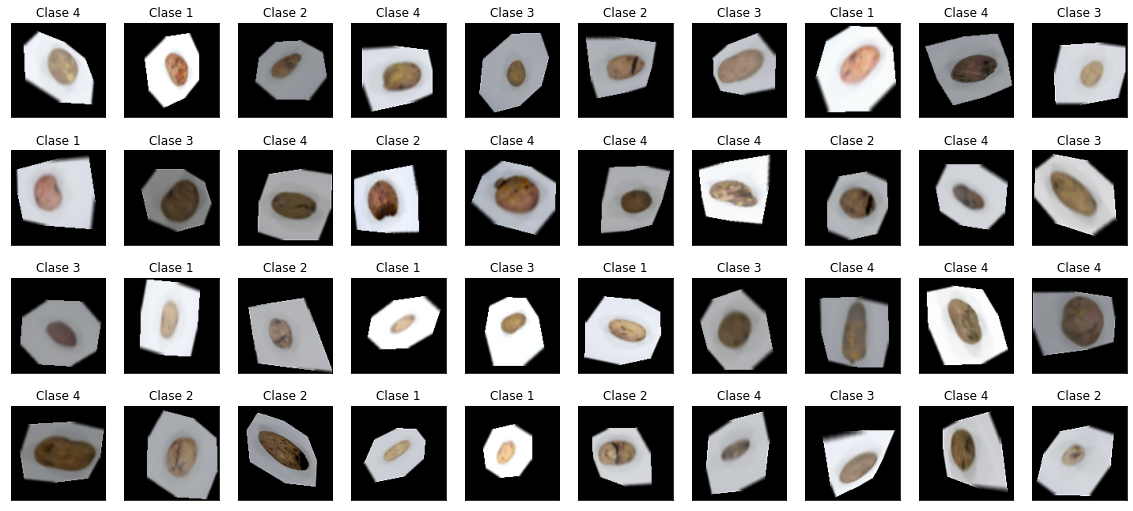
\includegraphics[scale=0.4]{Figs/augmentation.png}
				\caption{Matriz de Imágenes Con Transformaciones Aplicadas}
				\label{fig:agumentation}
			\end{figure}	

		\subsection{Funciones PotatoDataset y DataLoader}
		Aquí se presenta la creación de la función \textit{PotatoDataset()}, y la implementación de la función \textit{Dataloader}, ademas de la explicación de cada función.
		
		
			\subsubsection{FUNCIÓN POTATODATASET}
			
			Se creó una clase, (\textit{Python Class Object Constructor}), con el nombre de \textit{AttributesDataset()}, que se encarga de leer el \textit{Metadata}  de cada imágen y convertirlo en \textit{labelID}, en la Tabla \ref{table:metadata} se muestra como son ingresadas las imágenes en el algoritmo, sin embargo, las características deben ser ingresadas como \textit{labelID}, es decir, el label Pastusa corresponde al ID 0 en la categoría de Tipo. Este diccionario se presenta a continuación:			
	
			\begin{itemize}
				\item Tipo: ${'Pastusa': 0, 'R12': 1}$
				\item Daño: ${'Buena': 0, 'Defectuosa': 1}$
				\item Tamaño: ${'Muy Grande': 0, 'Grande': 1, 'Mediana': 2}$
			\end{itemize}

			En la red neuronal, únicamente se utilizaron \textit{labels} y \textit{labelID} de tipo y daño para definir las clases de la Tabla \ref{table:Clases}. La función \textit{Dataset} de \textit{Python} realiza el proceso de cargar y relacionar cada imágen con su respectivo \textit{label}, para \textit{Dataset's} que se encuentran organizados dentro de carpetas jerarquicamente. El \textit{Dataset} creado en éste documento no se encuentra organizado de esta manera, sino que la organización jerárquica que define las clases se encuentra dentro del \textit{metadata}, en el nombre de cada imágen, Tabla \ref{table:metadata}, debido esto es que se desarrolló una función que cargara y relacionara de la misma manera que lo hace la función integrada de \textit{Pythorch}. Esta función fue llamada \textit{PotatoDataset()}, que utiliza los \textit{labelID} generados por la función \textit{AttributesDataset()}, y carga cada imágen relacionada con sus \textit{labelID}. Como se desarrolló la función, de igual forma debe ser capaz de aplicar las transformaciones a cada imágen. El objeto regresa las 592 imágenes cargadas en \textit{Python}, cada una relacionada con su respectivo \textit{labelID} y \textit{label}, y con una transformación o múltiples aplicadas. Esta función desarrollada, cuenta con los mismos atributos iterables que poseen los \textit{dataset's} creados a partir de la función integrada en \textit{Pytorch}.			
			
		
			\subsubsection{FUNCIÓN DATALOADER}			
						
			Generalmente, una vez se finaliza el proceso de cargar las imágenes utilizando la función \textit{DataSet} de \textit{Pytorch}, se procede a utilizar la función \textit{DataLoader} para generar múltiples lotes de imágenes, a partir de las transformaciones utilizadas. La función \textit{DataLoader()}, de \textit{Pytorch}, es implementada para realizar la importación de datos a gran escala. Para el uso de esta función se debe tener en cuenta que el argumento más importante será el \textit{dataset}, que fue generado por el objeto \textit{PotatoDataset()}. \\
			
			Según como se explico en el apartado anterior, se generó un \textit{dataset} del tipo \textit{iterable-style Datsets}, lo que permite utilizar la función integrada \textit{DataLoader()} de \textit{Pytorch}. El \textit{DataLoader} permite la agrupación automática de muestras de datos individuales obtenidas en los \textit{Batch's} mediante argumentos. Los \textit{DataLoader's} cuentan con una gran catidad de argumentos que ayudan a que la carga de datos sea más eficiente \cite{Pytorch}. Es por esta razón, que para la ejecución de este dataloader se implementaron los parámetros de la Tabla \ref{table:Argumentos}.
			
			\begin{table}[ht]
				\centering
				\begin{tabular}{|p{3cm}|p{8cm}|}
					\hline
					FUNCIÓN & DESCRIPCIÓN \\ 
					\hline
					Batch size & Cuántas muestras por Batch hay que cargar (Default: 1)\\
					\hline
					Shuffle & Se establece en TRUE para que los datos se reorganicen en cada época (Default: FALSE)  \\
					\hline
					Num workers & Cuántos subprocesos se utilizarán para la carga de datos. 0 significa que los datos se cargarán en el proceso principal. (Default: 0)\\
					\hline
				\end{tabular}	
				\caption{Argumentos para el Dataloader}
				\label{table:Argumentos}
			\end{table}
		
		Los argumentos explicados en la tabla \ref{table:Argumentos} fueron establecidos de la siguiente forma:
		
		\begin{itemize}
			\item $Batch \ Size = 40$
			\item $Shuffle = True$
			\item $Num \ workers = 0$
		\end{itemize}

		Esto con el objetivo de que el \textit{Dataloader} cargue 40 muestras por época, y tome otras 40 diferentes para la siguiente época, y así sucesivamente hasta terminar todas las épocas establecidas.  
		
		
		
			
		
		\subsection{Hiperparámetros Del Modelo}
		
		Los hiperparámetros de un modelo son los valores de las configuraciones utilizadas durante el proceso de entrenamiento.
		
			\subsubsection{FUNCIÓN DE PÉRDIDAS}		
			
			\textit{Pytorch} posee una cantidad interesante de funciones de pérdidas, para su uso la clasificación de clases en redes neuronales. Una función de pérdidas, evalúa la desviación entre las predicciones realizadas por la red neuronal y los valores reales de las muestras utilizadas durante el entrenamiento de la red. Cuanto menor sea el valor de la función, es más eficiente la red neuronal \cite{mathivet2018inteligencia}. 	
			Para el desarrollo de la red neuronal, se utilizó la pérdida de entropía cruzada entre la entrada y el objetivo \cite{Pytorch}. Es útil cuando se entrena un problema de clasificación con más de una clase.  El objetivo que espera este criterio debe contener:
			
			\begin{itemize}
				\item Índices de clase en el rango $[0,C)$ donde $C$ es el número de clases.
				\item Probabilidades de clase se requieren más allá de una sola clase cuando se encuentran etiquetas combinadas.				 
			\end{itemize}
			
			En cada \textit{lote} usado en el entrenamiento de la red neuronal, se encuentran etiquetas combinadas en el \textit{Metadata} de las imágenes, como se describió en la Tabla \ref{table:Clases}, por lo tanto, una función de pérdida no reducida \cite{Pytorch} se describe en la Ecuación 5-4.\\
			
			\begin{equation}
				{l_n=-\sum_{c=1}^{C}w_c log\left(\frac{exp(x_n,c)}{\sum_{i=1}^{C}exp(x_n,i)}y_n,c\right)}
			\end{equation}\\
			
			Donde $x$ es la entrada, $y$ el objetivo de predicción, $w$ es el peso, $C$ el número de clases y $N$ es la dimensión del \textit{Batch}. Usando la función \textit{nn.CrossEntropyLoss()}, se calculan las pérdidas entre entrada y salida del modelo entrenado, para posteriormente utilizar estas pérdidas como métricas en porcentajes de \textit{Accuracy} y \textit{Losses}.\\
			
			
			El rendimiento de esta función de pérdidas, es mejor cuando el objetivo contiene índices de clase y no las etiquetas, ya que esto permite optimizar el cálculo, por esta razón, se agruparon las etiquetas de las imágenes en $4 \ Clases$ definidas.
			
			
			
			
			\newpage
			\subsubsection{OPTIMIZADOR}
			
			\textit{Pytorch} posee \textit{torch.optim}, que es un paquete que implementa varios algoritmos de optimización. 
			
			
			
			
			

			
			
		\subsection{Optimización Bayesiana}
		La mayor parte de modelos implementados en machine learning poseen una serie de parámetros que no pueden ser aprendidos de los datos, es por esto que deben ser establecidos antes del entrenamiento. Estos parámetros son conocidos como hiperparámetros.	
		\\
		Dos de las estrategias más empleadas para probar diferentes combinaciones y evaluarlas mediante métodos de validación, son \textit{grid search y random search}. En la primera estrategia, los valores estudiados de cada hiperparámetro son distribuidos de forma uniforme dentro de un rango delimitado por el analista. En la segunda estrategia, los datos son aleatorios dentro de ese rango como se muestra en la Figura \ref{fig:Hiperparámetros grid search y random search}	(REFERENCIA).
		
		\begin{figure}[ht]
			\centering
			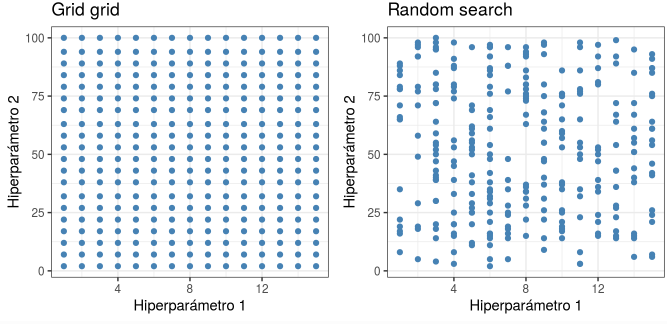
\includegraphics[scale=0.4]{Figs/121.png}
			\caption{Hiperparámetros grid search y random search}
			\label{fig:Hiperparámetros grid search y random search}
		\end{figure}
		
		A pesar de que las dos estrategias son válidas y se obtienen buenos resultados, sobretodo cuando se tiene criterio para acotar el rango de búsqueda, poseen una carencia similar: ninguna de las dos tiene en cuenta los resultados obtenidos hasta el momento, lo cual impide que se focalicen en la búsqueda de las regiones de mayor interés y evitando las regiones innecesarias.()
		\\
		Teniendo en cuenta lo descrito anteriormente, se procede a implementar la optimización bayesiana, la cual consiste en crear un modelo probabilístico en el que el valor de la función objetivo es la métrica de validación del modelo, (rmse, auc, precisión, etc). Con este método, se logra que la búsqueda se vaya redirigiendo en cada iteración hacia las regiones de mayor interés. Esto con el fin de reducir el número de combinaciones de los hiperparámetros con los que el modelo es evaluado, seleccionando únicamente los mejores candidatos. Esto significa que, la ventaja frente a las estrategias descritas anteriormente, se maximiza cuando el espacio de búsqueda es muy amplio o la evaluación del modelo es muy lenta.()
			
		\subsection{Arquitectura del modelo}
		Aquí se presenta la estructura y los resultados obtenidos de los modelos preentrenados AlexNet, VGG-19, VGG-11 y ResNet-18 sin optimizar.
			\subsubsection{\MakeUppercase{Modelo preentrenado ALEXNET}}
			
				El modelo AlexNet fue implementado en el año 2012 en el desafió de reconocimiento visual a gran escala Imaget. Este modelo tuvo un resultado tan satisfactorio que los modelos de aprendizaje profundo se convirtieron en la referencia para la investigación y desarrollo en los principales sectores de la industria. \cite{Pytorch}\\
				
				
				El modelo se compone de cinco capas convolucionales y tres capas densas, donde las capas convolucionales están normalizadas por lotes. El kernel tiene dimensiones diferentes que se distribuyen en \textit{11 x 11} en la primera capa, \textit{5 x 5} en la segunda y \textit{3 x 3} en las demás. La primera, cuarta y quinta capa convolucional están seguidas por una capa Max-pooling con dimensiones de \textit{3 x 3}, que posee un stride de dos.\\
				
				
				Las capas convolusionales y de Max-pooling son seguidas por tres capas densas, en donde las dos primeras poseen 4096 neuronas cada una y la ultima capa es la de salida, la cual se compone de 1000 neuronas que poseen una función de activación softmax. Estas neuronas son las encargadas de realizar la clasificación de la imagen. Como es habitual en estos sistemas de clasificación, la función de perdidas implementada es la entropía cruzada \cite{ref_1}.
				\\
				
				\begin{figure}[ht]
					\centering
					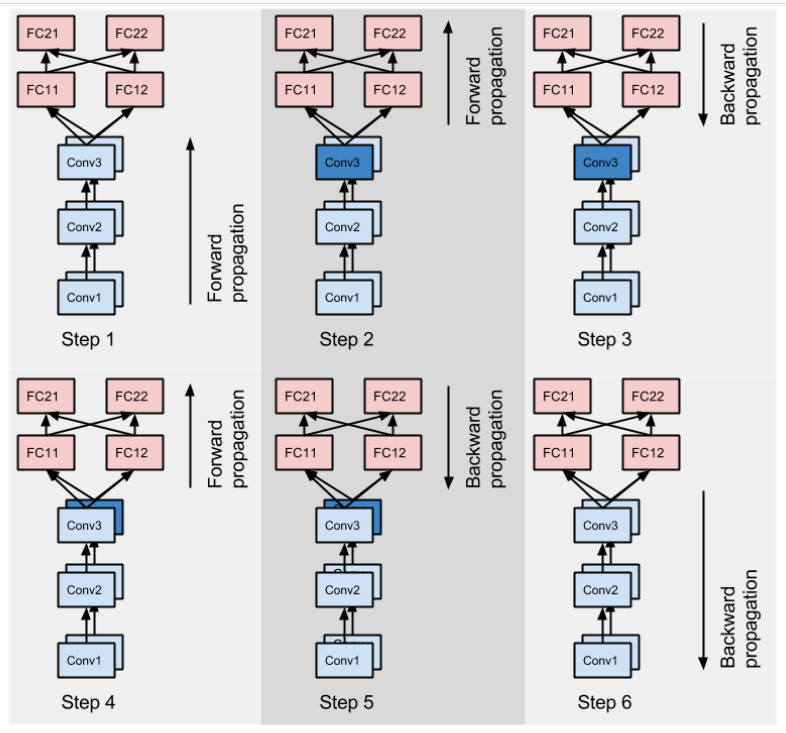
\includegraphics[scale=0.4]{Figs/5.png}
					\caption{Modelo AlexNet}
					\label{fig:AlexNet}
				\end{figure}
				\newpage	
				Como se aprecia en la Figura \ref{fig:AlexNet}, el modelo de AlexNet, toma una imagen de entrada con una resolución de \textit{227 x 227} pixeles y 3 canales de color, la información recibida pasa por cinco capas convolucionales, (en negro), de neuronas ReLu y tres capas de Max-pooling, (en azul). La quinta capa de convolución posee 256 mapas diferentes con dimensiones de \textit{13 x 13}. Seguidamente se aplican las dos capas densas de 4096 neuronas, las cuales son seguidas por una capa de salida de 1000 neuronas, dotadas con una función softmax. Cada neurona de la capa de salida representa un conjunto semántico diferente. Y su valor de activación indica la probabilidad de que la imagen de entrada pertenezca a dicho conjunto semántico.\\
		
				
				
				
\newpage

			\subsubsection{\MakeUppercase{Modelo preentrenado VGG19}}
			
				La arquitectura VGG fue planteada por Simonyan y Zisserman, la cual consiste en stacks lineales de bloques, que se encuentran formados por una cantidad determinada de capas convolucionales, una función de activación no lineal y una capa Max Pooling, seguidos de tres capas fully-conected y finalmente una capa softmax \cite{ref_2}. Esta arquitectura cuenta con cinco bloques los cuales están distribuidos como se muestra en la Figura \ref{fig:VGG19}.
				
				
				\begin{figure}[ht]
					\centering
					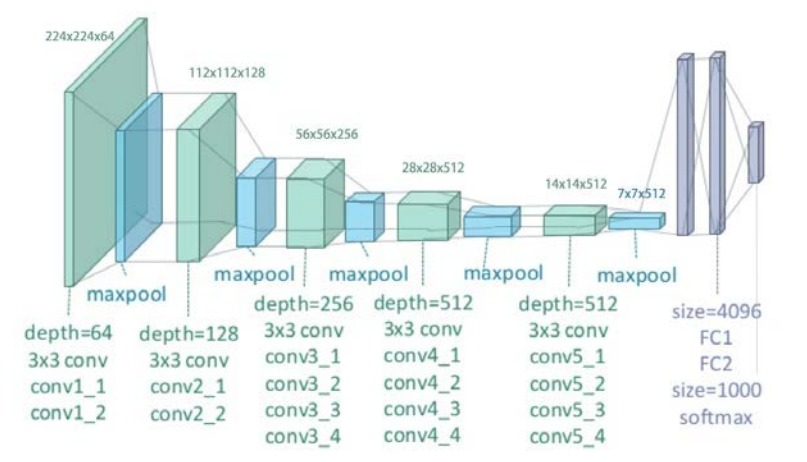
\includegraphics[scale=0.45]{Figs/22.jpeg}
					\caption{Modelo VGG19}
					\label{fig:VGG19}
				\end{figure}			
				
				
				Como se puede observar, la arquitectura cuenta con dos capas convolucionales de 64 y 128 filtros respectivamente, en sus dos primeros bloques, el bloque intermedio se compone de tres capas convolucionales de 256 filtros, y los últimos dos bloques están compuestos por tres capas concolucionales de 512 filtros cada uno. El numero 19 representa la cantidad de capas entrenables que posee la arquitectura, donde hay 16 capas convolucionales y 3 capas fully-conected.\\
\newpage				
				Las capas convolucionales de esta arquitectura cuentan con un campo receptivo de \textit{3 x 3}, stride de \textit{1 x 1} y pading de 1 pixel. Para la operaciones del Max Pooling se implementa un kernel de \textit{2 x 2} y un stride de \textit{2 x 2}, y por ultimo cada capa oculta de la red cuenta con la función de activación ReLu. La arquitectura VGG19 se resume en la Figura \ref{fig:VGG19_tabla}.
				
				\begin{figure}[ht]
					\centering
					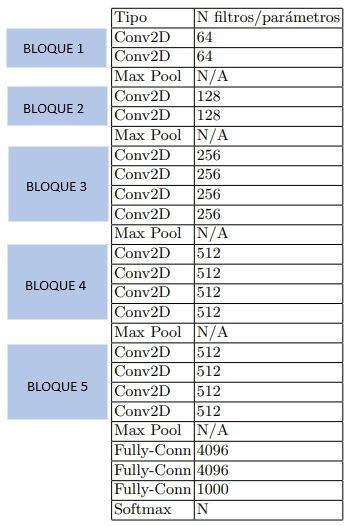
\includegraphics[scale=0.6]{Figs/21.jpeg}
					\caption{Composición Modelo VGG19}
					\label{fig:VGG19_tabla}
				\end{figure}

\newpage
				Ya que se conoce la forma en que esta estructurado el modelo, se procede a mostrar la precisión del algoritmo antes de ser aplicada la optimización bayesiana.
				
				\begin{figure}[ht]
					\centering
					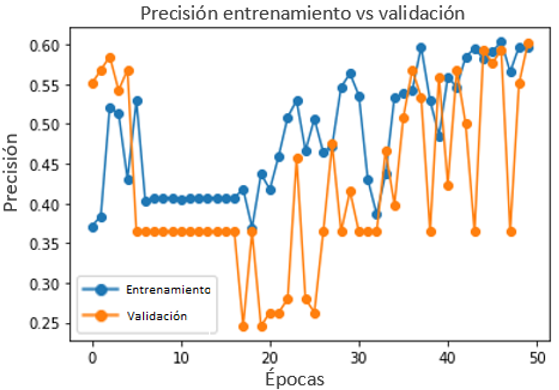
\includegraphics[scale=0.55]{Figs/101.png}
					\caption{Accuracy Modelo VGG19}
					\label{fig:VGG19_accuracy}
				\end{figure}  
				
				Como se puede observar en la Figura \ref{fig:VGG19_accuracy}, la precisión del modelo al completar 50 épocas es inferior al 60.
				\\
				En la Figura \ref{fig:VGG19_losses}, se puede apreciar que el modelo cuenta con \textit{16 \%} aproximadamente de desviación entre las predicciones y los valores reales, implementados durante el entrenamiento del modelo.
				
				\begin{figure}[ht]
					\centering
					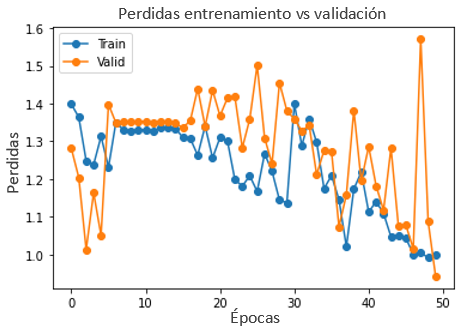
\includegraphics[scale=0.55]{Figs/102.png}
					\caption{Losses Modelo VGG19}
					\label{fig:VGG19_losses}
				\end{figure}
			
			Teniendo en cuenta la información presentada en las Figuras \ref{fig:VGG19_accuracy} y \ref{fig:VGG19_losses}, se puede apreciar que modelo presenta \textit{overfiting} durante el transcurso de las épocas 18 hasta la época 30, y finalmente culminada la época 50 del modelo, el porcentaje de \textit{overfiting} es aproximadamente cero, y se procede a presentar en la Figura \ref*{fig:VGG19_prediccion} la predicción realizada por el modelo.
			
				\begin{figure}[ht]
					\centering
					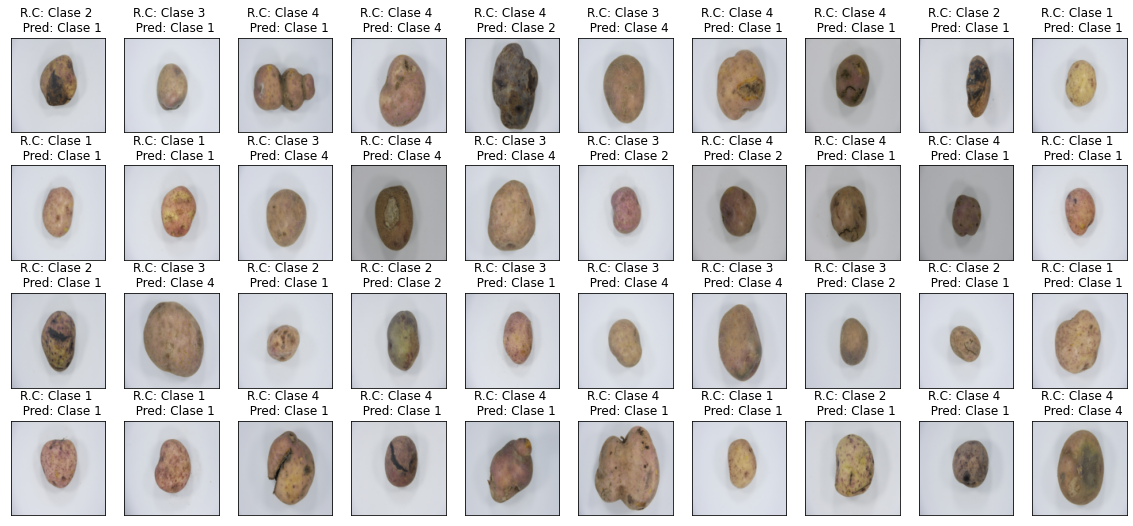
\includegraphics[scale=0.35]{Figs/103.png}
					\caption{Predicción Modelo VGG19}
					\label{fig:VGG19_prediccion}
				\end{figure}
		
		Se genera la matriz de confusión para validar los verdaderos positivos, verdaderos negativos, falsos positivos y falsos negativos, y se plasman en la Figura \ref{fig:MC_VGG19}.
		
				\begin{figure}[ht]
					\centering
					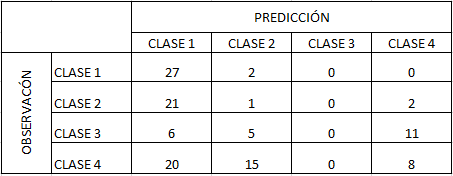
\includegraphics[scale=0.55]{Figs/131.png}
					\caption{Matriz de confusión modelo VGG19}
					\label{fig:MC_VGG19}
				\end{figure}
			
		Para finalizar en la Figura \ref{fig:ACU_VGG19}, se presenta la precisión del modelo VGG-19 por clase.
		
				\begin{figure}[ht]
					\centering
					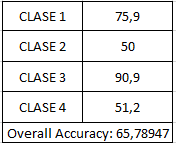
\includegraphics[scale=0.70]{Figs/132.png}
					\caption{Precisión por clase modelo VGG19}
					\label{fig:ACU_VGG19}
				\end{figure}
\newpage
			\subsubsection{\MakeUppercase{Modelo preentrenado VGG11}}
			VGG es un modelo preentrenado, en un conjunto de datos que contiene el peso que representan las características del conjunto de datos entrenados. Los modelos VGG toman una imagen de entrada de dimensiones \textit{224 x 224} pixeles en formato RGB, que son tratadas con un tamaño de imagen constante.
			\\
			 El modelo de aprendizaje profundo VGG11. Es la configuración mas sencilla. Tiene 11 capas de peso en total, de ahí el nombre VGG11. 8 de ellas son capas convolucionales y 3 son capas completamente conectadas, como se aprecia en la Figura \ref{fig:VGG11} \cite{ref_3}.
			
			\begin{figure}[ht]
				\centering
				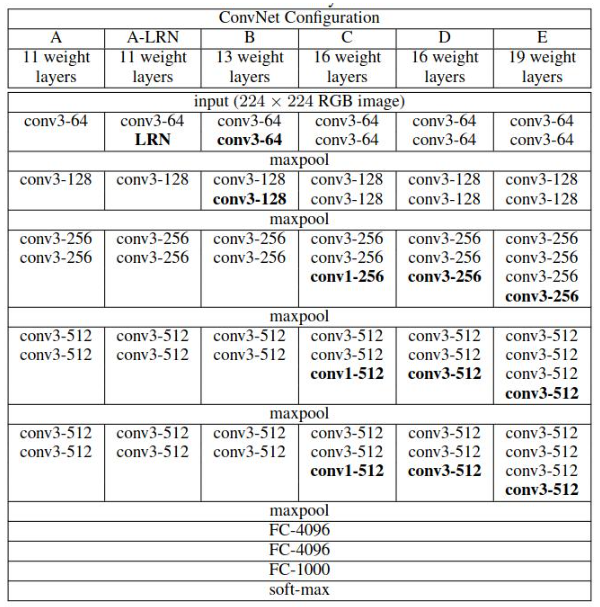
\includegraphics[scale=0.8]{Figs/70.png}
				\caption{Composición Modelo VGG-11}
				\label{fig:VGG11}
			\end{figure}
\newpage			
			Las 11 capas del modelo VGG11 son:
				\begin{itemize}
					\item Convolución usando 64 filtros + Max Pooling
					\item Convolución usando 128 filtros + Max Pooling
					\item Convolución usando 256 filtros
					\item Convolución usando 256 filtros + Max Pooling
					\item Convolución usando filtros 512
					\item Convolución usando 512 filtros + Max Pooling
					\item Convolución usando filtros 512
					\item Convolución usando 512 filtros + Max Pooling
					\item Totalmente conectado con 4096 nodos
					\item Totalmente conectado con 4096 nodos
					\item Capa de salida con activación Softmax con 1000 nodos.
				\end{itemize}
			
			El modelo cuenta con 11 capas ponderadas, sus pesos representan la fuerza de las conexiones entre unidades de capas de red adyacentes, son implementadas con el fin de conectar cada neurona de una capa con todas las neuronas de la siguiente capa, se debe tener en cuenta que la capa MAX-POOLING no se considera como una capa ponderada, debido a que es un mapa de características que contiene las características más destacadas.
			\\
			 El Max-Pooling es una operación de pooling que calcula el valor máximo que contiene cada parche en cada mapa de características, como resultado se obtiene mapas de características muestreados que destacan la característica más relevante en el parche, en la practica se ha comprobado que este método, es más eficiente que la agrupación media en tareas de visión por ordenador como la clasificación de imágenes.
\newpage

			Una vez conocida la forma en que se estructura el modelo VGG-11, se procede a evaluar su precisión antes de ser aplicada la optimización bayesiana y durante 50 épocas.
			
			\begin{figure}[ht]
				\centering
				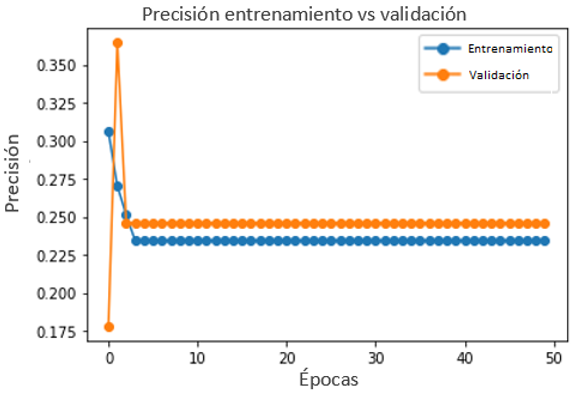
\includegraphics[scale=0.5]{Figs/105.png}
				\caption{Precisión Modelo VGG-11}
				\label{fig:precision_VGG11}
			\end{figure}
			
			Como se evidencia en la Figura \ref{fig:precision_VGG11}, el modelo cuenta con una precisión que ronda el 25 \%.
			\begin{figure}[ht]
				\centering
				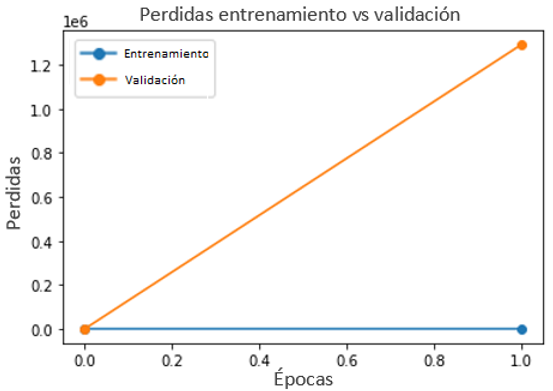
\includegraphics[scale=0.5]{Figs/106.png}
				\caption{Losses Modelo VGG-11}
				\label{fig:loses_VGG11}
			\end{figure}
			
			En la Figura \ref{fig:loses_VGG11}, se aprecia que el modelo cuenta con una desviación bastante significativa, entre las predicciones y los valores reales.
			\\
			\\
			Gracias a la información brindada por las figuras anteriores se deduce que el sistema posee un alto porcentaje de \textit{overfiting} que no puede ser corregido en el transcurso de las épocas.
\newpage
			\begin{figure}[ht]
				\centering
				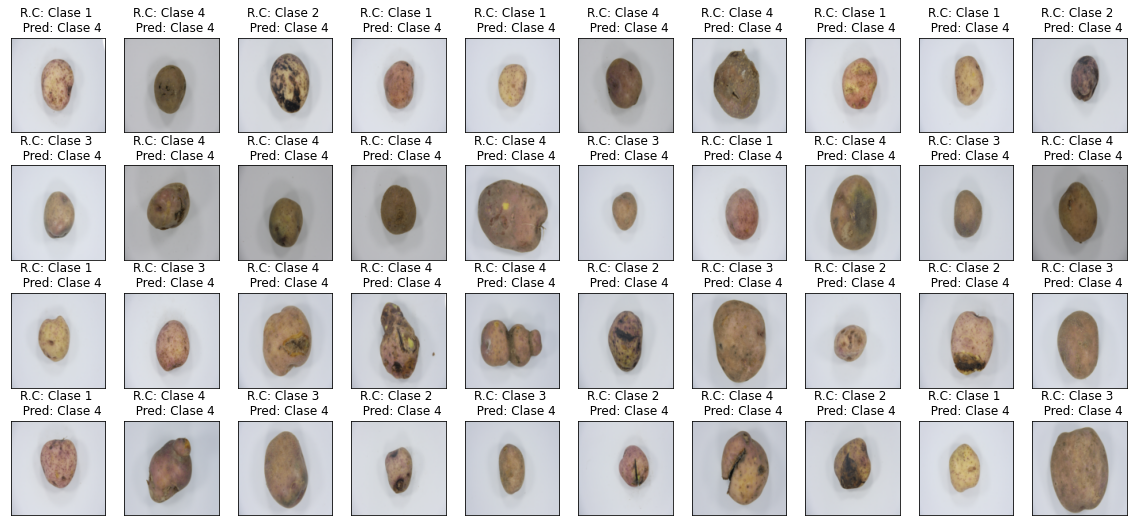
\includegraphics[scale=0.35]{Figs/107.png}
				\caption{Predicción Modelo VGG-11}
				\label{fig:Pre_VGG11}
			\end{figure}
			
			En la Figura \ref{fig:Pre_VGG11}, se presenta la predicción del modelo VGG-11 con las muestras implementadas para su validación.
			
			\begin{figure}[ht]
				\centering
				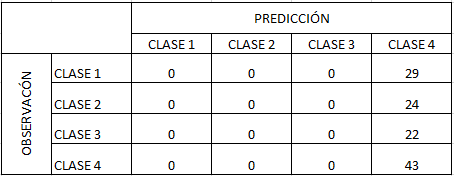
\includegraphics[scale=0.55]{Figs/51.png}
				\caption{Matriz de confusión Modelo VGG-11}
				\label{fig:MC_VGG11}
			\end{figure}
			
			La figura \ref{fig:MC_VGG11}, se presenta la matriz de confusión del modelo VGG-11, donde se aprecian los verdaderos positivos, verdaderos negativos, falsos positivos y falsos negativos.
			\\
			Para finalizar, la precisión de clasificación del modelo VGG-11 por clases sin optimización bayesiana se presenta en la Figura \ref{fig:clase_VGG11}.  
			
			\begin{figure}[ht]
				\centering
				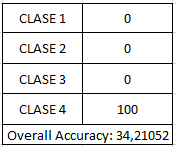
\includegraphics[scale=0.6]{Figs/52.png}
				\caption{Precisión por clase Modelo VGG-11}
				\label{fig:clase_VGG11}
			\end{figure}
\newpage
			\subsubsection{\MakeUppercase{Modelo preentrenado RESNET18}}
				La arquitectura Resnet, (Residual Net), fue propuesta por un equipo de Microsoft Research el cual fue liderado por Kaiming He, en donde se propone que si a una red neuronal de 20 capas se le intercalan 36 capas que calculan la simple función de identidad, la red resultante, (56 capas), debería tener exactamente la misma eficacia y no ser inferior que la primera. Debemos recordar que la función identidad es la encargada de devolver exactamente el mismo valor que su argumento \cite{ref_4}.
				\\
				Conociendo esto para permitir que una red pueda variar su cantidad efectiva de capas, se introduce el concepto de bloque residual:
	
				\begin{figure}[ht]
					\centering
					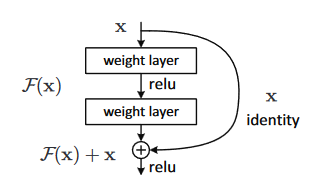
\includegraphics[scale=0.6]{Figs/67.png}
					\caption{Bloque Residual}
					\label{fig:Bloque}
				\end{figure}
			
				Como se aprecia en la Figura \ref{fig:Bloque}, el bloque residual se compone de una ruta residual, (izquierda), y una conexión atajo, (derecha), que la soslaya. La ruta residual F(x), esta compuesta de dos capas de pesos sinapticos, (pueden ser densas o convolucionales), que se intercalan por una función rectificadora. El resultado se suma con la información que atraviesa la conexión atajo \textit{X "identidad"}. Y por ultimo se aplica nuevamente la función rectificadora. La información puede atravesar con ello dos caminos diferentes que son: el de la función de identidad X o el de la ruta residual \textit{F(x)} \cite{ref_5}

\newpage

				En la arquitectura Resnet18, Las 18 capas de esta arquitectura representan las 18 capas con pesos, en donde se incluye la capa de convolución y la capa totalmente conectada, excluyendo la capa de agrupación y la capa BN.
				
				\begin{figure}[ht]
					\centering
					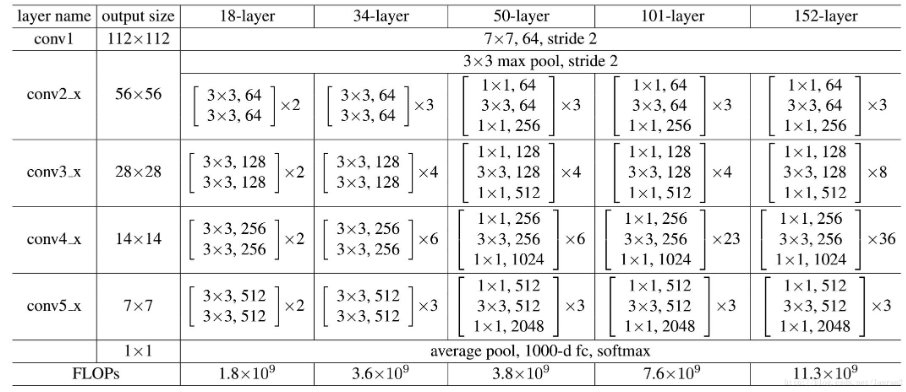
\includegraphics[scale=0.65]{Figs/68.png}
					\caption{Arquitectura ResNet18}
					\label{fig:ArqRes18}
				\end{figure}
				
				Como se puede observaren la Figura \ref{fig:ArqRes18}, la primera capa de convolución implementa una plantilla de \textit{7 x 77 x 7}, con un tamaño de paso de 2 y un relleno de 3, Seguido a eso, se realiza BN, ReLu y Maxpooling. Estos constituyen la primera parte del modulo de convolucion conv1.
				\\
				Luego hay cuatro etapas, cada etapa tiene múltiples módulos, cada módulo se llama un bloque de construcción, por ende se tiene que ResNet=[2,2,2,2] se evidencia que hay 8 bloques de construcción, como se presenta en la Figura \ref{fig:RESNET18} \cite{ref_5}.
\newpage				
				\begin{figure}[ht]
					\centering
					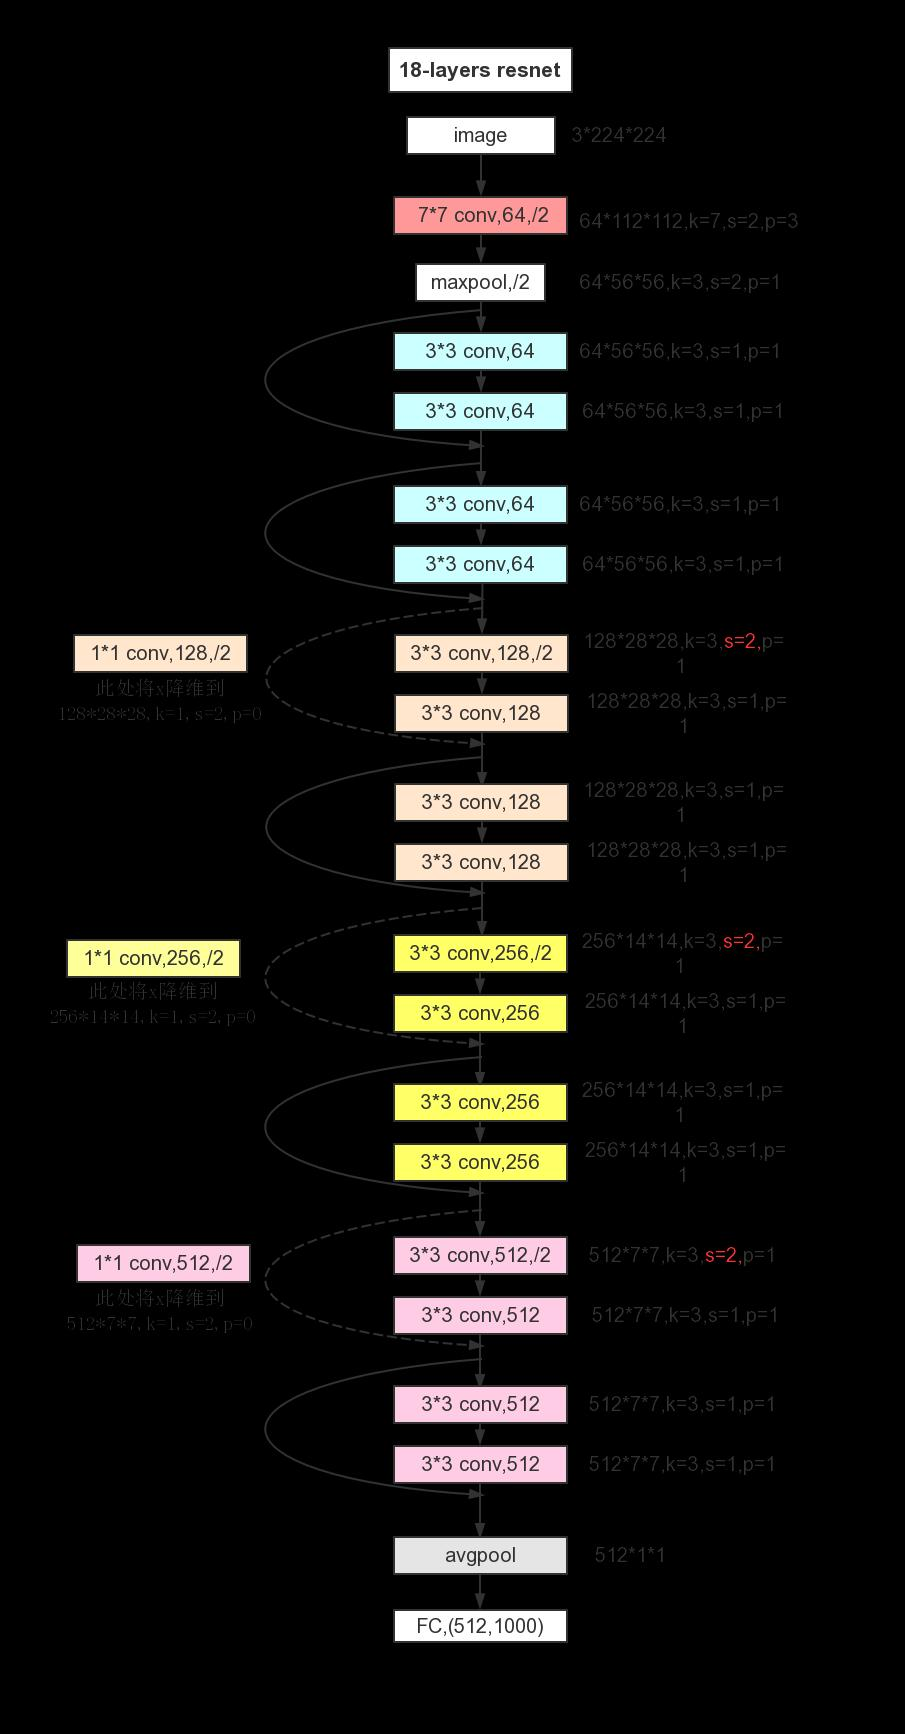
\includegraphics[scale=0.25]{Figs/69.png}
					\caption{Arquitectura Resnet18}
					\label{fig:RESNET18}
				\end{figure}

\newpage	
		En la Figura \ref{fig:preci_RESNET18}, se procede a presentar la precisión obtenida del modelo ResNet-18 durante 50 épocas, sin haber aplicado la optimizacion bayesiana.
		
		\begin{figure}[ht]
			\centering
			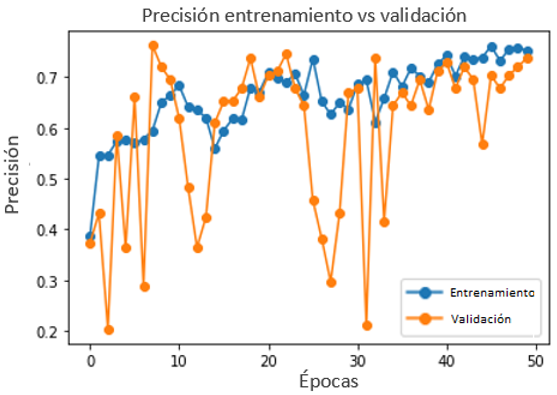
\includegraphics[scale=0.5]{Figs/109.png}
			\caption{Precisión modelo Resnet-18}
			\label{fig:preci_RESNET18}
		\end{figure}
	
		La información presentada en la Figura \ref{fig:perdda_RESNET18}, permite observar que el modelo cuenta con una desviación muy baja entre las predicciones y los valores reales, permitiendo concluir que el modelo cuenta con un bajo porcentaje de \textit{overfiting}. 
		
		\begin{figure}[ht]
			\centering
			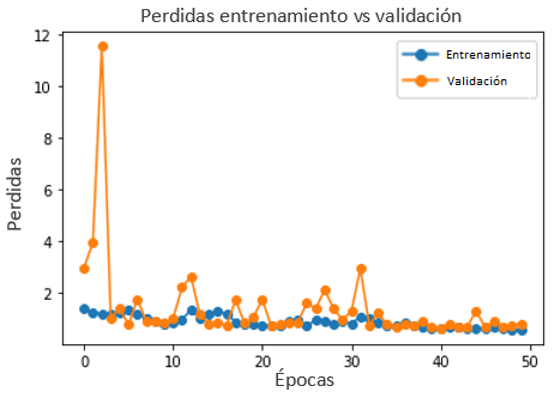
\includegraphics[scale=0.5]{Figs/110.png}
			\caption{Perdidas modelo Resnet-18}
			\label{fig:perdda_RESNET18}
		\end{figure}

\newpage
	La Figura \ref{fig:pre_RESNET18}, presenta las predicciones realizadas por el modelo ResNet-18 con las muestras implementadas durante su validación.
	
	\begin{figure}[ht]
		\centering
		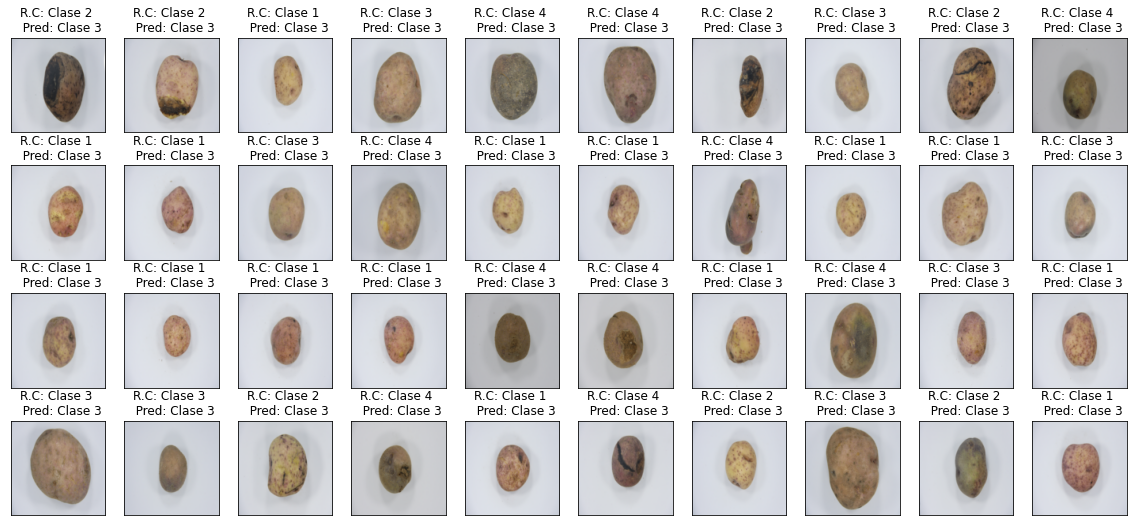
\includegraphics[scale=0.35]{Figs/111.png}
		\caption{Predicción modelo Resnet-18}
		\label{fig:pre_RESNET18}
	\end{figure}

	La matriz de confusión del modelos ResNet-18 es presentada en la Figura \ref*{MC_RESNET18}, con el fin de dar a conocer los verdaderos positivos, verdaderos negativos, falsos positivos, y falsos negativos del modelo
	
	\begin{figure}[ht]
		\centering
		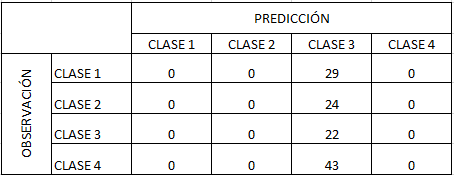
\includegraphics[scale=0.55]{Figs/71.png}
		\caption{Matriz de confusión modelo ResNet-18}
		\label{MC_RESNET18}
	\end{figure}
		 	
	Para finalizar, en la Figura \ref{clase_RESNET18}, se presenta la precisión del modelo sin optimización bayesiana por clases.
	
	\begin{figure}[ht]
		\centering
		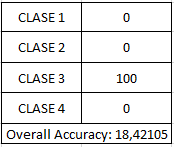
\includegraphics[scale=0.60]{Figs/72.png}
		\caption{Precisión por clase modelo ResNet-18}
		\label{clase_RESNET18}
	\end{figure}
	
			\subsubsection{\MakeUppercase{Comparación de arquitecturas}}
\newpage		
	\section{Clasificación de tamaño}
		La clasificación de los tubérculos de papa mediante su tamaño, (diámetro), se realiza para categorizar el producto bajo la norma técnica colombiana NTC 341 establecida por la industria alimentaria, con el fin de garantizar la calidad de los tubérculos de consumo.
		\\
		La norma establece cuatro categorías para la clasificación de los tubérculos mediante la medición de su tamaños, estas categorías se presentan en la Tabla \ref{table:limites}:
		
	\begin{table}[ht]
		\centering
		\begin{tabular}{|c|c|}
			\hline
			DENOMINACIÓN & DIÁMETRO (mm) \\
			\hline
			MUY GRANDE & MAYOR DE 90 \\
			\hline
			GRANDE & 65-90 \\
			\hline
			MEDIANA	& 45-64 \\
			\hline
			PEQUEÑA & 30-44 \\
			\hline
		\end{tabular}	
		\caption{Clases Limites tamaño de tubérculos de consumo}
		\label{table:limites}
	\end{table}	
	
\newpage
\chapter{Prototipo}
	En este capitulo se presentan diferentes numerales para detallar y explicar el prototipo implementado para la clasificación de tubérculos de papa. En el numeral \textit{6.1} se dan a conocer las especificaciones de la maquina implementada. seguido en el numeral \textit{6.2} se realiza la descripción de la maquina. En el numeral \textit{6.3} se tiene la descripción del sistema eléctrico y sus componentes, y por ultimo se termina con los numerales \textit{6.4 y 6.5} donde se explica la estructura construida para la clasificación de los tubérculos, y se finaliza con el funcionamiento de la maquina.
	
	\section{Especificaciones principales}
		Se implementa una banda transportadora tomada de una maquina selladora de banda continua horizontal FR-900, la cual es impulsada por un motor DC a 220V.
		Las especificaciones técnicas de la selladora de banda continua horizontal RF-900 se presentan en la Figura \ref{fig:principales}.
		
		\begin{figure}[ht]
			\centering
			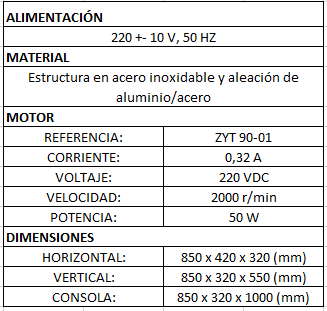
\includegraphics[scale=0.75]{Figs/13.png}
			\caption{Especificaciones Principales}
			\label{fig:principales}
		\end{figure}
		
	
\newpage
	\section{Descripción de la maquina}
		En la Figura \ref{fig:Banda}, se presenta un esquema general de la maquina selladora de banda continua horizontal FR-900, y en la Tabla \ref{table:Banda} se describen las partes presentadas en la Figura \ref{fig:Banda}.
		\begin{figure}[ht]
			\centering
			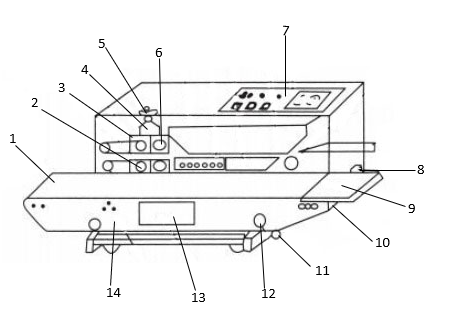
\includegraphics[scale=0.95]{Figs/65.png}
			\caption{Maquina Banda Transportadora}
			\label{fig:Banda}
		\end{figure}
	
		\begin{table}[ht]
			\centering
			\begin{tabular}{|p{5cm}|p{8cm}|}
				\hline
				1- Cinta transportadora & 8- Enchufe de corriente y protección \\ 
				\hline
				2- Rueda de goma& 9- Mesa de trabajo fija\\
				\hline
				3- Rodillo de goma& 10- Tornillo de regulación de la elasticidad de las cintas transportadoras\\
				\hline
				4- Asiento rueda de tintorería& 11- Perilla de regulación de la entrada y salida de la estación de transporte\\
				\hline
				5- Rueda reguladora de presión& 12- Perilla de regulación de la altura de la estación transportadora\\
				\hline
				6- Rueda motriz& 13- Placa de identificación\\
				\hline
				7- Caja de Control& 14- Estación de transporte\\
				\hline
			\end{tabular}	
			\caption{Descripción Maquina Transportadora}
			\label{table:Banda}
		\end{table}

\newpage
	\section{Esquema eléctrico}
		En la Figura \ref{fig:Esquema} se presenta las conexiones eléctricas realizadas para el funcionamiento del prototipo, ademas de esto se anexa en la Tabla \ref{table:esquema} el listado de elementos implementados.  
		\begin{figure}[ht]
			\centering
			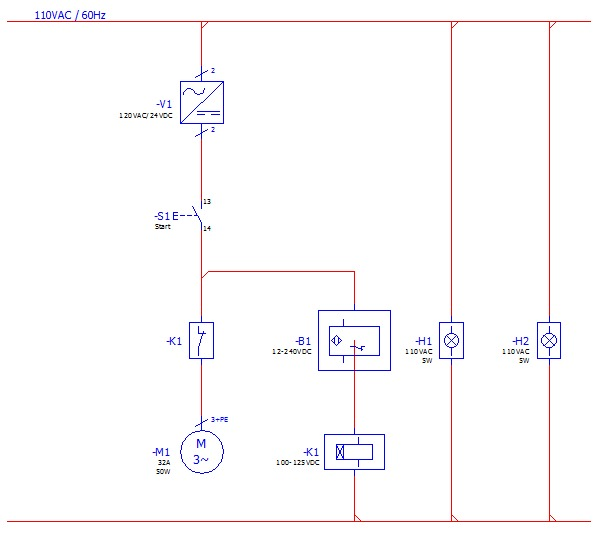
\includegraphics[scale=0.5]{Figs/66.jpg}
			\caption{Esquema eléctrico}
			\label{fig:Esquema}
		\end{figure}
	
		\begin{table}[ht]
		\centering
		\begin{tabular}{|p{2cm}|p{5cm}||p{3cm}|}
			\hline
			SÍMBOLO & NOMBRE & CANTIDAD \\ 
			\hline
			 V1 & Fuente de Voltaje & 1 \\
			\hline
			 S1 & Pulsador & 1 \\
			\hline
			 K1 & Timer & 1 \\
			\hline
			 M1 & Motor DC & 1 \\
			\hline
			 B1 & Sensor Fotoeléctrico & 1 \\
			\hline
			 H1 & Bombillos & 2 \\
			\hline
		\end{tabular}	
		\caption{Elementos Esquema Eléctrico}
		\label{table:esquema}
		\end{table}	
		
\newpage	
	\section{Estructura}
		La caja elaborada para el análisis de los tubérculos de papas, fue construida en acetato con medidas de, \textit{35 x 25(cm)} las laminas frontal y trasera, \textit{16 x 25(cm)} lamina superior, \textit{20 x 16(cm)} laminas laterales como se muestra en las Figuras.
	
		Como se muestra en las Figuras , las laminas fueron diseñadas con las medidas necesarias que permitan posicionar algunos elementos necesarios para realizar la clasificación de los tuberculos, como lo son bombillos, un sensor optico y una camara web, los cuales seran definidos en los numerales \textit{6.4.1, 6.4.2 y 6.4.3}.
		\subsection{Bombillos}
			La estructura cuenta con dos agujeros donde se ubican dos bombillos de luz blanca de 6500 Kelvin de temperatura de color para mantener la iluminación fija a una distancia de 30cm de todas las fotos al igual que se tomaron durante la construcción del Dataset.
		\subsection{Sensor Fotoeléctrico}
			Se implementa un sensor fotoeléctrico, de referencia MAGEWAY, el cual tiene como objetivo detener la banda transportadora una vez el tubérculo de papa se encuentre posicionado bajo la cámara, para realizar su respectiva inspección, el sensor cuenta con las siguientes especificaciones.
			\\
			\\
			\textbf{ESPECIFICACIONES TÉCNICAS:}
				\begin{itemize}
					\item Método de detección: retroreflectante.
					\item Ángulo: 1,5 o aprox.
					\item Máx. Rango de detección: 4 m.
					\item Voltaje de alimentación: 12-240 VDC, 24-240V ACBR, Salida: Relé SPDT
					\item Capacidad de salida: 3 A/30 VCC, 3 A/250 VAC.
					\item Temperatura ambiente: -4-131 °F (-20-55 °C).
				\end{itemize}
\newpage			
		\subsection{Cámara Web}
			Para la detección de los tubérculos de papa, se implementa una cámara \textit{Web Camera America Store}, la cual será la encargada de la toma de fotos de los tubérculos, mientras son transportados en la banda transportadora para su análisis.
			\\
			\\
			\textbf{ESPECIFICACIONES TÉCNICAS:}
			\begin{itemize}
				\item Lente: Lente de Cristal
				\item Tamaño del artículo: 8 x 4 x 8 cm
				\item Chip DSP: sin controlador
				\item Sensor de imagen: CMOS
				\item Resolución dinámica: 1920 x 1080
				\item Marco: 30 fps
				\item Longitud Focal: 8 mm - infinity
				\item Longitud del Cable: aproximadamente 138 cm
			\end{itemize}
			
	\section{Funcionamiento}
		













